\documentclass{uofsthesis-cs}
\usepackage{graphicx}
\graphicspath{ {./images/c2/}, {./images/c3/}, {./images/}, {./images/appendix/ai/}}
\usepackage{amssymb}
\usepackage{amsmath}
\usepackage{changes}
\usepackage{bm}
\definechangesauthor[name=Dave Schneider, color=red]{djs}
\definechangesauthor[name=Yujie Pei, color=green]{Yuge}
\usepackage{caption}
\usepackage{subcaption}
\usepackage{booktabs}
\usepackage{algorithmic} % package for generating algorithms
\setcounter{secnumdepth}{4}
\setcounter{tocdepth}{4}

\newcommand{\subsubsubsection}[1]{\paragraph{#1}\mbox{}\\}




\title{An Alternative Method for Characterization and Comparison of Plant Root Shapes}


\author{Yujie Pei}
\degree{\MSc}
\defencedate{Month/Year}
\department{School of Environment and Sustainability}
%\Academicunit{Master of Environment and Sustainability}



\begin{document}


% ___________________________ BEFORE THE BODY OF THESIS _______________

% baesed on https://students.usask.ca/graduate/thesis-preparation.php#ArrangementofContents

\maketitle % 1. Title Page

% 2. Permission to use and disclaimer Statement

%\abstract{}  % 3. abstract

%\acknowledgements{}  % 4. Acknowledgements

% 5. Permission to Reproduce 

%\dedication{}  % 6. Dedication

\tableofcontents % 7. Table of content

% 8. List of tables

% 9. List of figures

% 10. List of abbreviation



% 11. Body of the Thesis

% ___________________________ BODY OF THESIS _________________________

%%%%%%%%%%%%%%%%%%%%%%%%%% CHAPTER 1 %%%%%%%%%%%%%%%%%%%%%%%%%%%%%%%%%%

\chapter{Existing Morphological Descriptors for Root Systems}

  


\section{Background}

   \subsection{Importance of Roots}
      \begin{itemize}
        \item Mechanical and functional abilities of plant roots
        \item Plant root plasticity in the resource-limited environment
      \end{itemize}
      
     \subsection{Importance of Research}
       \subsubsection{Demand in crop breeding programs}
       \subsubsection{Environment and Sustainability}

         \begin{itemize}
           \item reduce the negative impacts of fertilization
           \item high crop productivity to feed the increasing global population
         \end{itemize}
         
       \subsection{Promising application in other branching structures}
         \begin{itemize}
           \item Trees
           \item River networks in geography
           \item Blood vessels in medicine
           \item Leaf vein networks
         \end{itemize}

  


\section{Summary of Existed Descriptors}
 
   \subsection{Metric}

     \subsubsection{Basic Geometric Descriptors}
       \begin{itemize}
         \item maximum depth
         \item maximum width
         \item etc.
       \end{itemize}
       
     \subsubsection{Compound Descriptors (Computed From the Basic Descriptors)}
       \begin{itemize}
         \item Density
         \item aspect ratio
         \item etc.
       \end{itemize}
       
     \subsubsection{Weaknesses}

       \begin{itemize}
         \item Rely on the resolution of the images \cite{balduzzi2017reshaping}
         \item Only provide a general view of root morphology \cite{balduzzi2017reshaping}
         \item Difficult to assess the spatial configuration of roots
         \item Fail to describe the full complexity of root systems
       \end{itemize}

       
   \subsection{Non-metric}
       
    \subsubsection{Topological Analysis}

      \begin{itemize}
        \item Persistent homology \cite{li2017persistent}
          \begin{itemize}
            \item Persistence barcode shows the number of branches.
            \item Persistence barcode indicates how branched roots connect along the scale of the function (e.g. geodesic distance).
            \item Compare the similarity of branching structures by a pair-wise distance matrix using the bottleneck distance method.
          \end{itemize}
          
       \item Horton-Strahler index \cite{toroczkai2001topological}
         \begin{itemize}
            \item Categorize the topological complexity of the whole branching structure.
            \item Provide a numerical measure of connectedness and complexity of the branching at each vertex by a dimensionless ratio: bifurcation ratio.
            \item The range of index and the length ratio indicate the size of the branching structure.
         \end{itemize}
                
       \item Fractal Analysis \cite{tatsumi1989fractal}
         \begin{itemize}
            \item Measure the complexity of branching structures.
            \item Measure self-similarity of branching structures by fractal dimension of the root systems.
         \end{itemize}
      \end{itemize}
      

   \subsubsection{Strengths}
     \begin{itemize}
       \item Highly complementary to geometric descriptors to characterize how individual roots are connected through branching \cite{delory2018archidart}.
       \item Describe branching structures independent of transformation and deformation.
     \end{itemize}
     

   \subsubsection{Problems and Weaknesses}
     \begin{itemize}  
       \item Only analyze the connectedness of branching structures, which is a portion of the complexity of plant root systems.
       \item Fail to characterize spatial distribution.
       \item Some biologically topological indices analyze the root growth qualitatively based on line-linked systems \cite{fitter1986topology}, but not characterize the mathematical topological properties.
       \item The fractal analysis aims to describe self-similar structures, which grow by continually repeating simple growth rules \cite{fitter1992fractal}.
     \end{itemize}
     

       

  \section{Problem Statements}


...
    %\2 Limitation of Data: large variance of length scales of root leads to the high requirement of the image resolution.
    %\2 Incompleteness and Low Efficiency
      %\3 The finite number of descriptors can not recover overall root system architecture.
      %\3 Diverse units of the measurement results in extra efforts in multivariate data analysis.
      %\3 Roots are not self-similar inherently.

      

  
  
%%%%%%%%%%%%%%%%%%%%%%%%%% CHAPTER 2 %%%%%%%%%%%%%%%%%%%%%%%%%%%%%%%%%%

\chapter{An Alternative Mathematical Method for Shape Description}

  %______________ Section 1: Kac’s Idea _______________________
  

\section{Kac’s Idea: Can One Hear the Shape of a Drum? \cite{kac1966can}}



  \subsection{Interpretations of Kac's Problem}

     \begin{itemize}
       \item When the drum vibrates, one can hear the sound, which is composed of tones of various frequencies. How much can shape features be inferred from hearing a discrete spectrum of pure tones produced by a drum?
       \item If a complete sequence of eigenvalues of the Dirichlet problem for the Laplacian can be obtained precisely, will people determine the shape of a planar?
     \end{itemize}




    \subsection{Problem Statement}

     \begin{itemize}     
       \item Consider a simply connected membrane $\Omega$ in the Euclidean space bounded by a smooth convex curve $\partial \Omega$ (e.g. a drum without any holes)
       \item Find function $\phi$ on the closure of $\Omega$, which vanishes at the boundary $\partial \Omega$, and a number $\lambda$ satisfying $-\Delta \phi = \lambda \phi$.

         \begin{itemize}
           \item $\Delta$ is the Laplace operator. e.g. $\Delta = \sum_{i=1}^{n} \frac{\partial ^2}{\partial x_i^2}$ in Cartesian coordinate system.
           \item If there exists a solution $\phi \neq 0$, the corresponding $\lambda$ is defined as a Dirichlet eigenvalue.
           \item For each domain $\Omega$, there has a sequence of eigenvalues $\lambda_1, \lambda_2, \lambda_3, ... $ corresponding to a set of eigenfunction $\phi_1, \phi_2, \phi_3, ...$.
           \item $\phi_k$ form an orthonormal basis of $L^2(\Omega)$ of real valued eigenfunctions; the corresponding discrete Dirichlet eigenvalues are positive ($\lambda_k \in \mathbb{R}^{+}$).
         \end{itemize}
         
       \item An important function \cite{grieser2013hearing}:

         \begin{equation}\label{eq:heat_trace}
           h(t) = \sum_{k=1}^{\infty} e^{-\lambda_kt}
         \end{equation}
         
         \begin{itemize}  
           \item It is a Dirichlet series.
           \item It is called the spectral function or the heat trace.
           \item It is smooth and converges for every $t>0$.
         \end{itemize}
     \end{itemize}



     \subsection{Summarize the Results of Kac's Idea}

       \begin{equation}\label{eq:kac_result}
          h(t) = \sum_{k=1}^{\infty} e^{-\lambda_kt} \sim \frac{|\Omega|}{2\pi t} - \frac{L}{4} \frac{1}{\sqrt{2\pi t}} + \frac{1}{6}
       \end{equation}
     
      \begin{itemize} 
        \item As $t \rightarrow 0^{+}$, the leading terms of the asymptotic expansion of $h(t)$ imply the geometrical attributes of $\Omega$
          \begin{itemize}
            \item the total area
            \item the perimeter
            \item the curvature
          \end{itemize}
          
        \item If the domain $\Omega$ has the polygonal boundary, the third term shows in the information about the interior angles of the polygon \cite{grieser2013hearing}.
      \end{itemize}



    \subsection{Conclusion}

     \subsubsection{Advantages}

        \begin{itemize}
          \item Kac proposed a novel analytical mathematical method for the shape description without using measuring tools, e.g. rulers.
          \item Other mathematicians extended Kac's idea in exploring the geometrical information of more complex domains with various boundary conditions \cite{khabou2007shape}\cite{gottlieb1985eigenvalues}\cite{gottlieb1983hearing} \cite{zayed1989heat}\cite{sleeman1984trace}.
        \end{itemize}
        
     \subsubsection{Limitations}
        
        \begin{itemize}
          \item It is only available for the convex domain, which has a smooth or piecewise smooth boundary.  
          \item Except in very few cases (i.e. rectangular, disk, certain triangles), the complete sequence of eigenvalues $\lambda_k$ can not be calculated \cite{grieser2013hearing}.
          \item Only the first few terms in the asymptotic expansion of $h(t)$ are explicitly available.
        \end{itemize}


    

%%%%%%%%%%%%%%%%%%%%%%%%%% CHAPTER 3 %%%%%%%%%%%%%%%%%%%%%%%%%%%%%%%%%%
  
\chapter{LRWs in Artificial Images}

  %______________ Section 1: Circle and Rectangle ______________
  
The fixed-time step Monte Carlo simulation, LRWs, has been validated
in the annulus in Appendix \ref{appendix:method_validation_annulus} by
comparing the analytical and numerical survival function. The further
validation of LRWs is to distinguish the geometries and explore their
structural features from both short and long time survival behaviours.



\section{\highlight[id=Yuge]{Circle and Rectangle}}

Given two simple convex shapes with the same area, circle and
rectangle, we are interested in how and whether their corresponding
survival curves differ from each other. For the equal-area geometries,
rectangle and circle, Eq. \ref{eq:kac_result} indicates that the
survival function of the former decays faster than the latter as the
time approaches zero.

The preliminary step of testing the research hypothesis is to generate
two black-and-white images with the same dimensions as shown in
Fig.~\ref{fig:simple_imgs}. In the binary images, circle and rectangle
have an equal number of white pixels. For simplicity, the centroid of
shapes located at the center of the image. Then, simulating LRWs in
the images and estimating survival functions by Kaplan-Meier
estimator.


 \subsection{Output Analysis}
 
   \begin{figure}
     \centering
     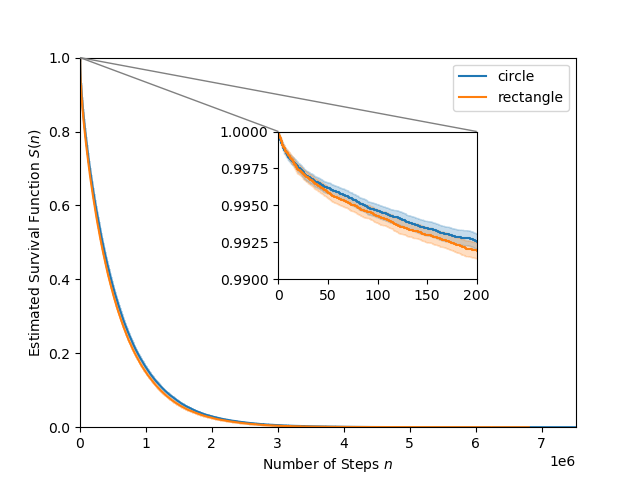
\includegraphics[width=\textwidth]{circle_rect_steps_sf.png}
     \label{fig:sf_simple_shape_steps}
     \caption{In the inset, the decay rate of the survival function for the rectangle is slightly larger than for the circle, which coincides with the theoretical result.}
   \end{figure}

  The differences between survival functions for the circle and
  rectangle are not visible. Moreover, the approximate $95\%$
  confidence intervals of the survival functions overlap. In this
  case, non-parametric statistical tests can be used to compare entire
  survival distributions and assess their dissimilarities. The logrank
  test has maximum power if the proportional hazards assumption is
  satisfied. 

   \begin{figure}
     \centering
     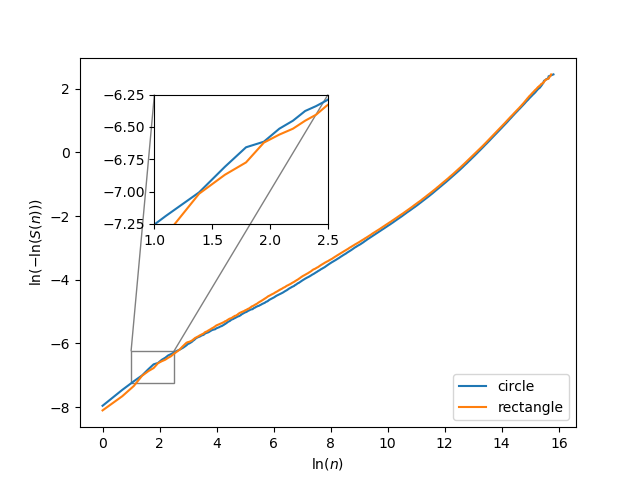
\includegraphics[width=\textwidth]{circle_rect_steps_ph.png}
     \label{fig:ph_test_simple_shapes}
     \caption{It is a graphical method for checking proportionality by looking for parallelism. As shown in the inset plot, two curves cross at some points and their shapes vary over time. Moreover, $p < 0.05$ in the non-proportional test. Thus, the survival functions for circle and rectangle do not satisfy the proportional hazard assumption.}
   \end{figure}


   \begin{table}
     \centering
     \begin{tabular}{lrr}
        \toprule
         {} &  test\_statistic &             p \\
         \midrule
         Logrank & 137.23 & 0.0 \\
         \midrule
         Tarone-Ware & 134.31 & 0.0 \\
         \midrule
         Gehan-Breslow & 123.83 & 0.0 \\
         \midrule
         Fleming-Harrington & 123.83 & 0.0 \\
         \bottomrule
     \end{tabular}
     \caption{Survival functions for circle and rectangle are statistically different since p values equal zeros.}
     \label{tab:test_simple_shape_steps}
   \end{table}



\subsection{Conclusion}


Although the proportional hazard assumption test is failed as shown in
Fig.~\ref{fig:ph_test_simple_shapes}, the weighted logrank tests
indicate that the null hypothesis should be rejected. In conclusion,
LRWs is an alternative tool to quantify and distinguish the geometries
in the $2-$ dimensional image without measuring the predefined shape
descriptors.
  


  %_______ Section 2: Complicated Branching Structures _________
  \section{Complicated Branching Structures}


   \subsection{Image Description}

     \begin{itemize}
         \item Image size: $1200 \times 1000$ pixels
         \item Surface area of shapes: $90000$ pixels
         \item Iterate the template $3, 4, 5, 6$ times to produce the targeted branching geometries labelled as $L_3, L_4, L_5, L_6$.
         \item Two groups of images labelled as $G_1, G_2$

           \begin{itemize}
             \item $G_1$: the target object $G_1 L_i$ ($i=3, 4, 5, 6$) is equidistant to the edges of an image.
             \item $G_2$: the template of $G_2 L_i$ ($i=3, 4, 5, 6$) is distinct from $G_1$ (thickness and aspect ratio). 
           \end{itemize}
           
     \end{itemize}



   \subsection{Output Analysis}


     \subsubsection{$S(n)$}



       \subsubsubsection{Estimated Survival Curves}

     
       \begin{figure}
        \centering
        
        \begin{subfigure}[b]{0.45\textwidth}
          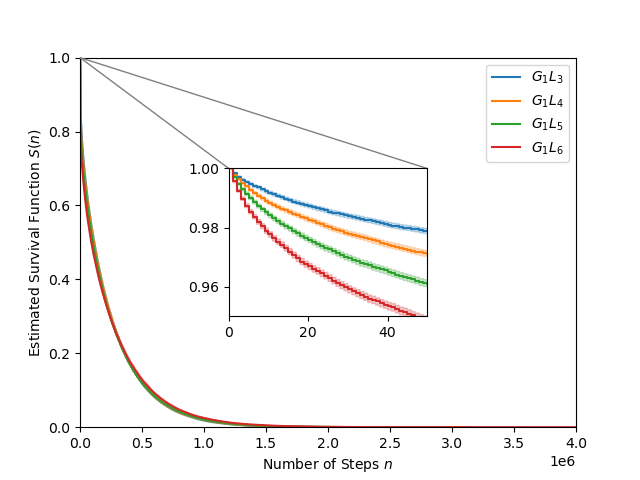
\includegraphics[width=\textwidth]{G_1_steps_sf.png}
          \caption{}
          \label{fig:sf_g1_branch_steps}
        \end{subfigure}
        \hfill
        \begin{subfigure}[b]{0.45\textwidth}
          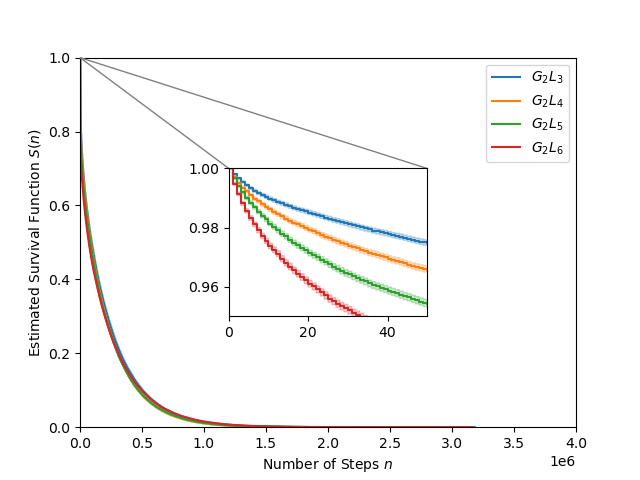
\includegraphics[width=\textwidth]{G_2_steps_sf.png}
          \caption{}
          \label{fig:sf_g2_branch_steps}
        \end{subfigure}

        \caption{}
        \label{fig:sf_branch_steps}

      \end{figure}



       \subsubsubsection{Non-Parametric Statistical Tests}

       
      \begin{table}
        \centering
        \begin{tabular}{llrrrr}
          \toprule
                       &             &         &  p &    &     \\
          \cmidrule{3-6}
                       &             & Logrank & TW & GB & FH  \\
          \midrule
          $G_1$ $L_3$  & $G_1$ $L_4$  &  0.4393 &  0.0285 &  0.0005 &  0.0005     \\
                       & $G_1$ $L_5$  & 0.0 & 0.0 & 0.0 & 0.0    \\
                       & $G_1$ $L_6$  & 0.0 & 0.0 & 0.0 & 0.0      \\
          $G_1$ $L_4$  & $G_1$ $L_5$  & 0.0007 & 0.0 & 0.0 & 0.0      \\
                       & $G_1$ $L_6$  & 0.0002 & 0.0 & 0.0 & 0.0       \\
          $G_1$ $L_5$   & $G_1$ $L_6$ & 0.7223 &  0.0 & 0.0 & 0.0      \\
          \bottomrule
        \end{tabular}
        \label{tab:g1_ingroup_tests_steps}
        \caption{}
      \end{table}


      \begin{table}
        \centering
        \begin{tabular}{llrrrr}
          \toprule
                       &             &         &  p &    &     \\
          \cmidrule{3-6}
                       &             & Logrank & TW & GB & FH  \\
          \midrule
          $G_2$ $L_3$  & $G_2$ $L_4$  &  0.0 &  0.0 &  0.0 &  0.0     \\
                       & $G_2$ $L_5$  & 0.0 & 0.0 & 0.0 & 0.0    \\
                       & $G_2$ $L_6$  & 0.0 & 0.0 & 0.0 & 0.0      \\
          $G_2$ $L_4$  & $G_2$ $L_5$  & 0.0016 & 0.0 & 0.0 & 0.0      \\
                       & $G_2$ $L_6$  & 0.0004 & 0.0 & 0.0 & 0.0       \\
          $G_2$ $L_5$   & $G_2$ $L_6$ & 0.7199 &  0.0 & 0.0 & 0.0      \\
          \bottomrule
        \end{tabular}
        \label{tab:g2_ingroup_tests_steps}
        \caption{}
      \end{table}



       \subsubsubsection{Mesurement of Dissimilarities for $S(n)$}
      

      \begin{figure}
        \centering
        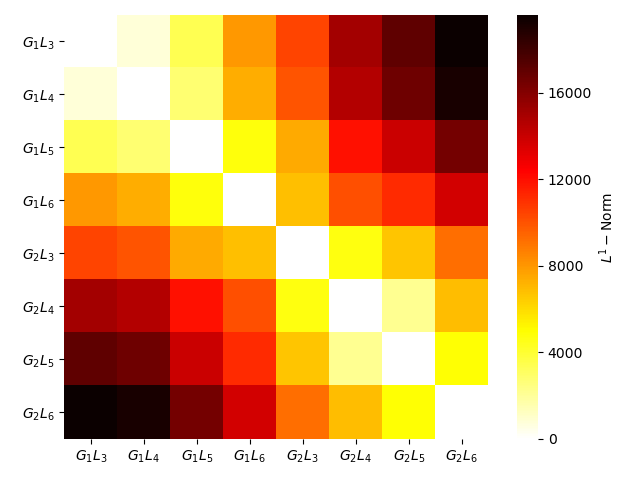
\includegraphics[width=\textwidth]{heatmap_ai_steps_l1.png}
        \caption{}
        \label{fig:heatmap_ai_steps_l1}
      \end{figure}

      
      \begin{figure}[h!]
        \centering
        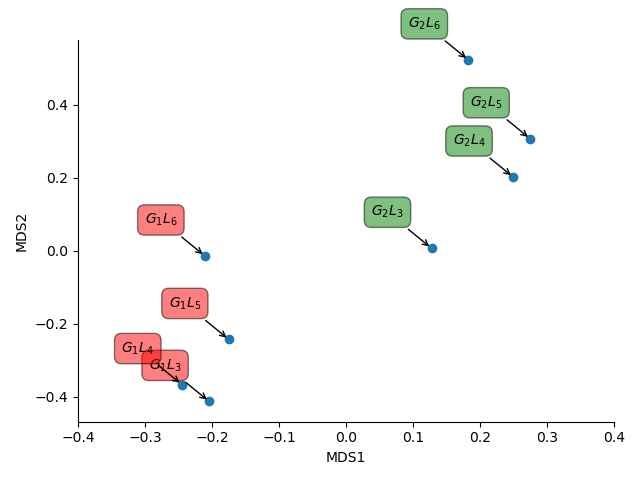
\includegraphics[width=\textwidth]{MDS_ai_steps_l1.png}
        \caption{}
        \label{fig:MDS_ai_steps_l1}
      \end{figure}
      


      
      \subsubsubsection{Visualize $S(n)$}

       \begin{figure}
         \centering
         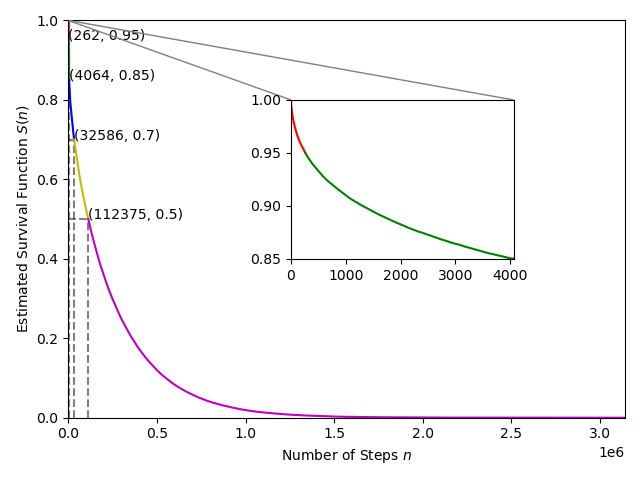
\includegraphics[width=\textwidth]{steps_seg_curve_G_1_L_3.png}
         \caption{}
         \label{fig:steps_seg_curve_G_1_L_3}
      \end{figure}



       \begin{figure}
         \centering
         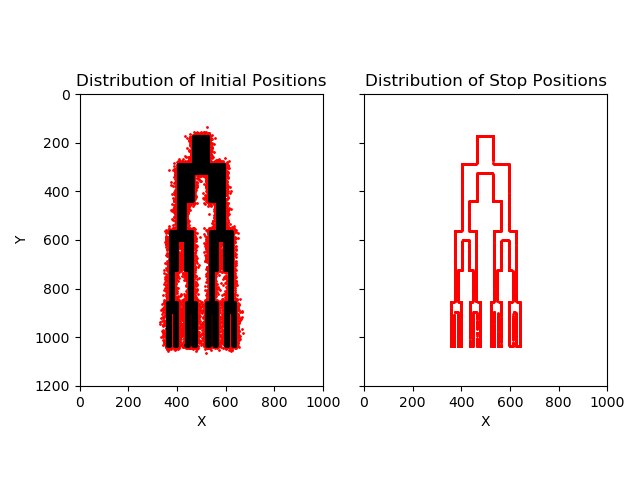
\includegraphics[width=\textwidth]{G_1_L_3_steps_red_initial_pos_distribution.png}
         \caption{}
         \label{fig:G_1_L_3_steps_red_initial_pos_distribution}
       \end{figure}



       \begin{figure}
         \centering
         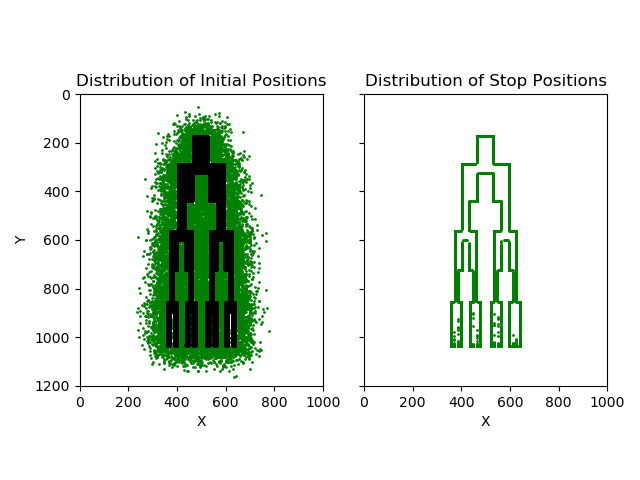
\includegraphics[width=\textwidth]{G_1_L_3_steps_green_initial_pos_distribution.png}
         \caption{}
         \label{fig:G_1_L_3_steps_green_initial_pos_distribution}
       \end{figure}


       \begin{figure}
         \centering
         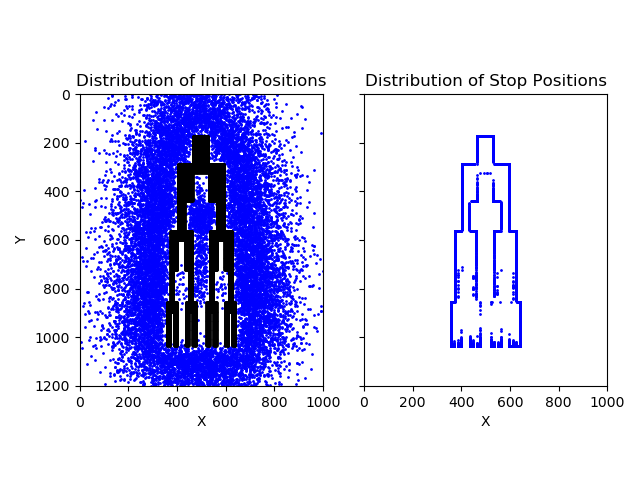
\includegraphics[width=\textwidth]{G_1_L_3_steps_blue_initial_pos_distribution.png}
         \caption{}
         \label{fig:G_1_L_3_steps_blue_initial_pos_distribution}
       \end{figure}
       

       \begin{figure}
         \centering
         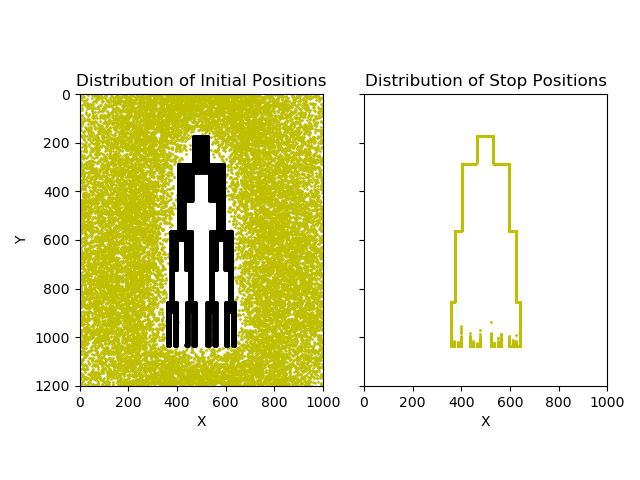
\includegraphics[width=\textwidth]{G_1_L_3_steps_y_initial_pos_distribution.png}
         \caption{}
         \label{fig:G_1_L_3_steps_y_initial_pos_distribution}
       \end{figure}


       \begin{figure}
         \centering
         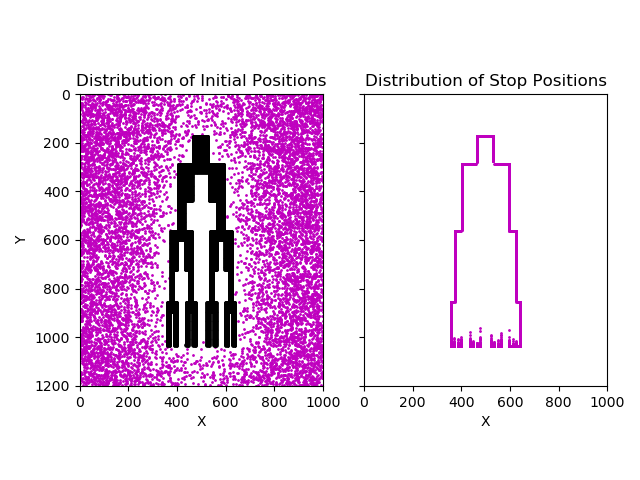
\includegraphics[width=\textwidth]{G_1_L_3_steps_m_initial_pos_distribution.png}
         \caption{}
         \label{fig:G_1_L_3_steps_m_initial_pos_distribution}
       \end{figure}


























      

      %____________________________________________________________



       \newpage

       
      \subsubsection{$S(d)$}



      \begin{figure}
        \centering
        
        \begin{subfigure}[b]{0.45\textwidth}
          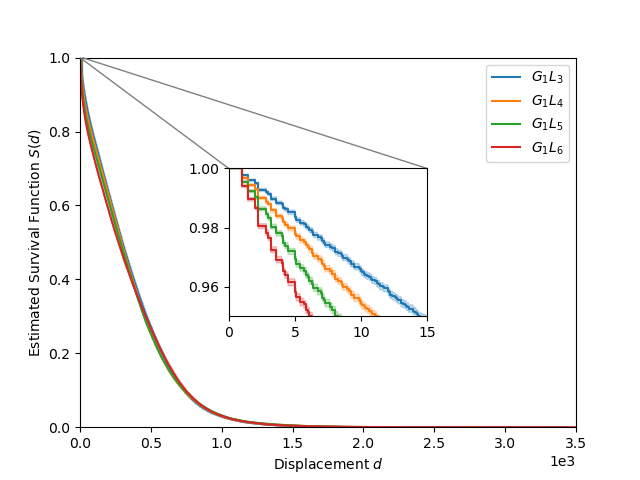
\includegraphics[width=\textwidth]{G_1_unwrap_disp_sf.png}
          \caption{}
          \label{fig:sf_g1_branch_disp}
        \end{subfigure}
        \hfill
        \begin{subfigure}[b]{0.45\textwidth}
          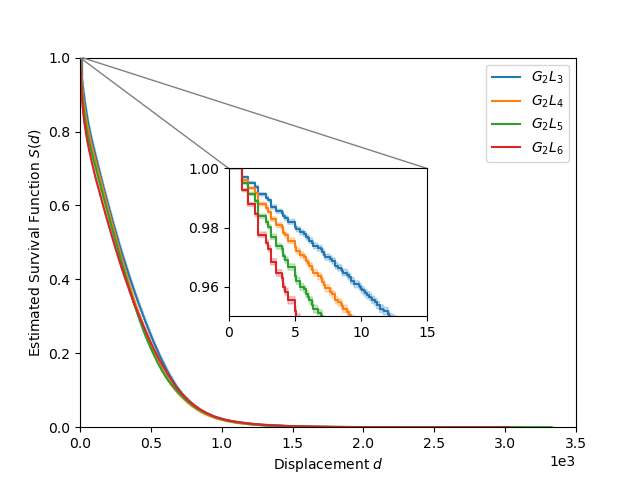
\includegraphics[width=\textwidth]{G_2_unwrap_disp_sf.png}
          \caption{}
          \label{fig:sf_g2_branch_disp}
        \end{subfigure}

        \caption{}
        \label{fig:sf_branch_disp}

      \end{figure}




      \begin{table}
        \centering
        \begin{tabular}{llrrrr}
          \toprule
                       &             &         &  p &    &     \\
          \cmidrule{3-6}
                       &             & Logrank & TW & GB & FH  \\
          \midrule
          $G_1$ $L_3$  & $G_1$ $L_4$  &  0.0 &  0.0 &  0.0 &  0.0     \\
                       & $G_1$ $L_5$  & 0.0 & 0.0 & 0.0 & 0.0    \\
                       & $G_1$ $L_6$  & 0.0 & 0.0 & 0.0 & 0.0      \\
          $G_1$ $L_4$  & $G_1$ $L_5$  & 0.0072 & 0.0 & 0.0 & 0.0      \\
                       & $G_1$ $L_6$  & 0.0003 & 0.0 & 0.0 & 0.0       \\
          $G_1$ $L_5$   & $G_1$ $L_6$ & 0.2883 &  0.0 & 0.0 & 0.0      \\
          \bottomrule
        \end{tabular}
        \label{tab:g1_ingroup_tests_disp}
        \caption{}
      \end{table}


      \begin{table}
        \centering
        \begin{tabular}{llrrrr}
          \toprule
                       &             &         &  p &    &     \\
          \cmidrule{3-6}
                       &             & Logrank & TW & GB & FH  \\
          \midrule
          $G_2$ $L_3$  & $G_2$ $L_4$  &  0.0 &  0.0 &  0.0 &  0.0     \\
                       & $G_2$ $L_5$  & 0.0 & 0.0 & 0.0 & 0.0    \\
                       & $G_2$ $L_6$  & 0.0 & 0.0 & 0.0 & 0.0      \\
          $G_2$ $L_4$  & $G_2$ $L_5$  & 0.0001 & 0.0 & 0.0 & 0.0      \\
                       & $G_2$ $L_6$  & 0.0015 & 0.0 & 0.0 & 0.0       \\
          $G_2$ $L_5$   & $G_2$ $L_6$ & 0.7019 &  0.0 & 0.0 & 0.0      \\
          \bottomrule
        \end{tabular}
        \label{tab:g2_ingroup_tests_disp}
        \caption{}
      \end{table}




      %______________________________________________________________
      

      \newpage
      

      \subsubsection{$S(R)$}
      
      \begin{figure}
        \centering
        
        \begin{subfigure}[b]{0.45\textwidth}
          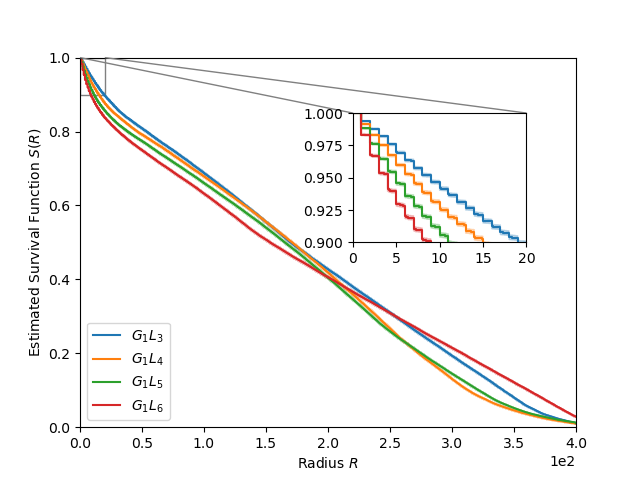
\includegraphics[width=\textwidth]{G_1_initial_radius_sf.png}
          \caption{}
          \label{fig:sf_g1_branch_radius}
        \end{subfigure}
        \hfill
        \begin{subfigure}[b]{0.45\textwidth}
          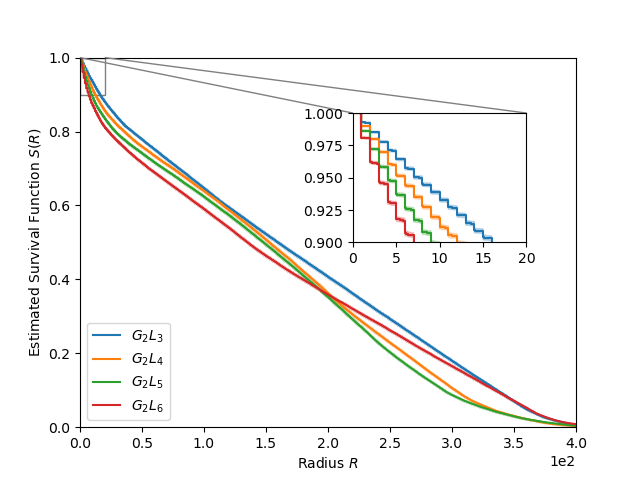
\includegraphics[width=\textwidth]{G_2_initial_radius_sf.png}
          \caption{}
          \label{fig:sf_g2_branch_radius}
        \end{subfigure}

        \caption{}
        \label{fig:sf_branch_radius}

      \end{figure}

      
      \begin{table}
        \centering
        \begin{tabular}{llrrrr}
          \toprule
                       &             &         &  p &    &     \\
          \cmidrule{3-6}
                       &             & Logrank & TW & GB & FH  \\
          \midrule
          $G_1$ $L_3$  & $G_1$ $L_4$  &  0.0 &  0.0 &  0.0 &  0.0     \\
                       & $G_1$ $L_5$  & 0.0 & 0.0 & 0.0 & 0.0    \\
                       & $G_1$ $L_6$  & 0.0 & 0.0 & 0.0 & 0.0      \\
          $G_1$ $L_4$  & $G_1$ $L_5$  & 0.1773 & 0.0 & 0.0 & 0.0      \\
                       & $G_1$ $L_6$  & 0.0 & 0.0 & 0.0 & 0.0       \\
          $G_1$ $L_5$   & $G_1$ $L_6$ & 0.0 &  0.0 & 0.0 & 0.0      \\
          \bottomrule
        \end{tabular}
        \label{tab:g1_ingroup_tests_radius}
        \caption{}
      \end{table}


      \begin{table}
        \centering
        \begin{tabular}{llrrrr}
          \toprule
                       &             &         &  p &    &     \\
          \cmidrule{3-6}
                       &             & Logrank & TW & GB & FH  \\
          \midrule
          $G_2$ $L_3$  & $G_2$ $L_4$  &  0.0 &  0.0 &  0.0 &  0.0     \\
                       & $G_2$ $L_5$  & 0.0 & 0.0 & 0.0 & 0.0    \\
                       & $G_2$ $L_6$  & 0.0 & 0.0 & 0.0 & 0.0      \\
          $G_2$ $L_4$  & $G_2$ $L_5$  & 0.0 & 0.0 & 0.0 & 0.0      \\
                       & $G_2$ $L_6$  & 0.0 & 0.0 & 0.0 & 0.0       \\
          $G_2$ $L_5$   & $G_2$ $L_6$ & 0.0 & 0.0 & 0.0253 & 0.0253      \\
          \bottomrule
        \end{tabular}
        \label{tab:g2_ingroup_tests_radius}
        \caption{}
      \end{table}


      


















    


      \newpage
      
    \subsection{Conclusion}

      \begin{itemize}
         \item In a short time, the survival function of rectangle decays faster than the circle, which conforms to the analytical results.
  
         \item The differences of estimated survival functions between circle and rectangle are statistically significant, which coincides with the real shape dissimilarities.

         \item Within a same group, when $t$ is small, the more branching the object is, the faster the survival function decays.

         \item Within a same group, the pairwise survival functions are statistically different.

         \item The corresponding target structures in $G_1$ and $G_3$ are invariant shapes under translation since their survival function are not statistically different. In other words, periodic boundary conditions of the image can eliminate the effect of the locations.

         \item LRWs can describe and classify the geometries, their spatial configurations, and the unoccupied area in the image.
    \end{itemize}





  


\subsection{\highlight[id=Yuge]{Output Analysis of $S(n)$}}

    
       \begin{figure}
        \centering 
        \begin{subfigure}[b]{0.45\textwidth}
          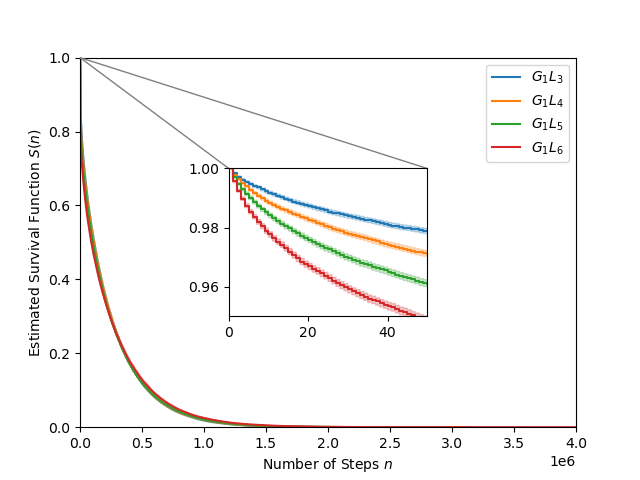
\includegraphics[width=\textwidth]{G_1_steps_sf.png}
          \caption{}
          \label{fig:sf_g1_branch_steps}
        \end{subfigure}
        \hfill
        \begin{subfigure}[b]{0.45\textwidth}
          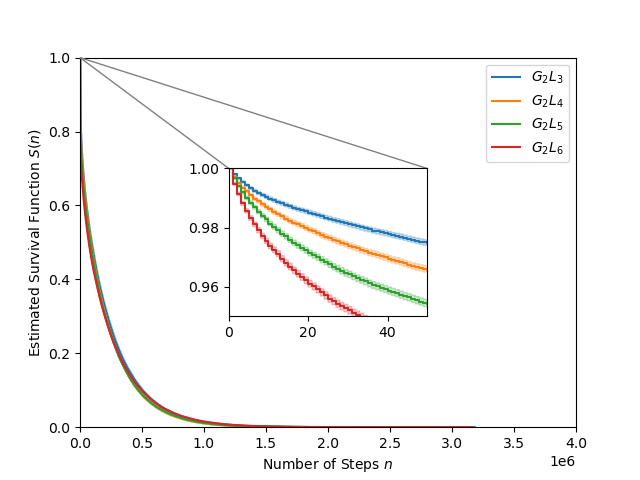
\includegraphics[width=\textwidth]{G_2_steps_sf.png}
          \caption{}
          \label{fig:sf_g2_branch_steps}
        \end{subfigure}
        \caption{(a) and (b) are survival functions for branching
          structures in $G_1$ and $G_2$, respectively. $n$ is the
          number of steps taken by the particle from the initial to
          the stop pixel in LRWs.}
        \label{fig:sf_branch_steps}
      \end{figure}

       
       The insets in Fig.~\ref{fig:sf_branch_steps} show that, within
       a group, the decay rates of $S(n)$ for $L_j$, $j=3, ..., 6$,
       are significantly distinct as $n$ approaches $0$. The graphical
       representation of short-time behaviours of survival functions
       is consistent with the analytical result since bigger $j$
       results in the larger perimeter of the branching structure.
       

       \begin{figure}
         \centering
         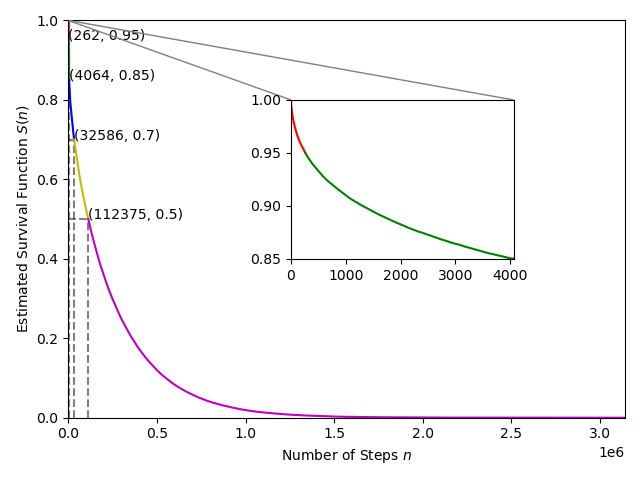
\includegraphics[width=\textwidth]{steps_seg_curve_G_1_L_3.png}
         \caption{It is an estimated survival function for LRWs in $G_1L_3$.}
         \label{fig:steps_seg_curve_G_1_L_3}
       \end{figure}

       
       As shown in Fig.~\ref{fig:steps_seg_curve_G_1_L_3}, the
       survival curve is divided into several coloured segments. In
       Fig.~\ref{fig:G_1_L_3_steps_red_initial_pos_distribution},
       Fig.~\ref{fig:G_1_L_3_steps_green_initial_pos_distribution},
       Fig.~\ref{fig:G_1_L_3_steps_blue_initial_pos_distribution},
       Fig.~\ref{fig:G_1_L_3_steps_blue_initial_pos_distribution}, and
       Fig.~\ref{fig:G_1_L_3_steps_pink_initial_pos_distribution},
       particles' initial and stop positions are painted with colour
       identical to the survival curve segment to understand the
       underlying stochastic process and its properties. Furthermore,
       the black region in the initial position plot is the target
       branching structure.

       
       
       \begin{figure}
         \centering
         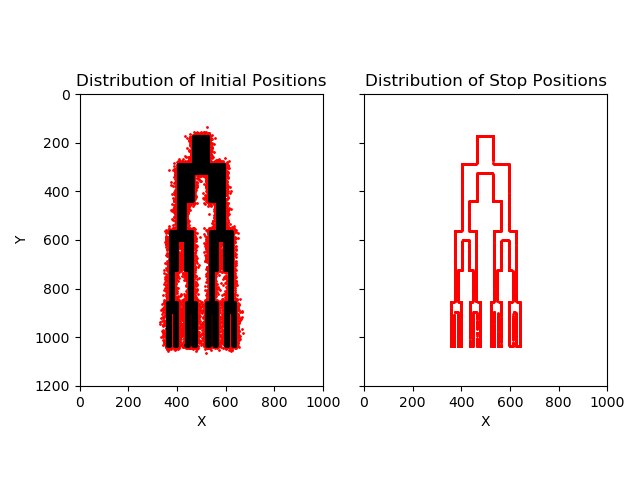
\includegraphics[width=\textwidth]{G_1_L_3_steps_red_initial_pos_distribution.png}
         \caption{$5\%$ of particles in the LRWs coloured by red will
           be absorbed within $262$ steps. In the left subfigure,
           particles' initial positions are distributed closely
           surrounding the target branching structure. The in-between
           space of tiny bottom limbs is filled with particles, while
           some area between the huge top branches is empty. The right
           subfigure shows that the red particles characterize the
           entire boundary of the object.}
         \label{fig:G_1_L_3_steps_red_initial_pos_distribution}
       \end{figure}



       \begin{figure}
         \centering
         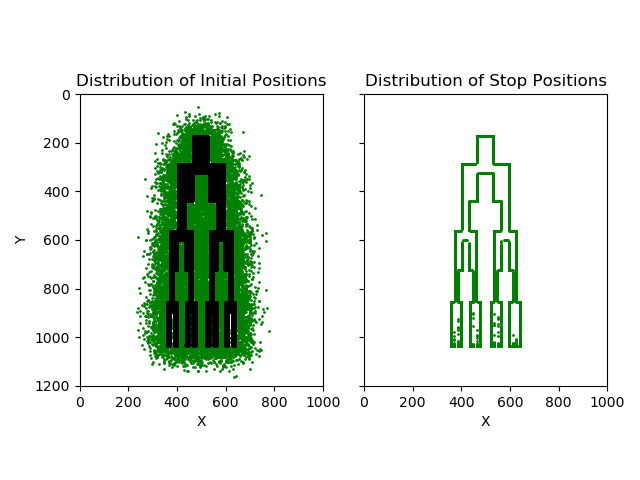
\includegraphics[width=\textwidth]{G_1_L_3_steps_green_initial_pos_distribution.png}
         \caption{Around $10$ percent of particles are generated
           adjacent to the fringe of the object, whose steps ranged
           from $262$ to $4064$. Compared with
           Fig.~\ref{fig:G_1_L_3_steps_red_initial_pos_distribution},
           the green points also dispersed thoroughly between the
           branches. Nevertheless, some in-between regions of the
           lowest branches are empty, resulting in the object's
           incompleted edge in the right plot.}
         \label{fig:G_1_L_3_steps_green_initial_pos_distribution}
       \end{figure}


       \begin{figure}
         \centering
         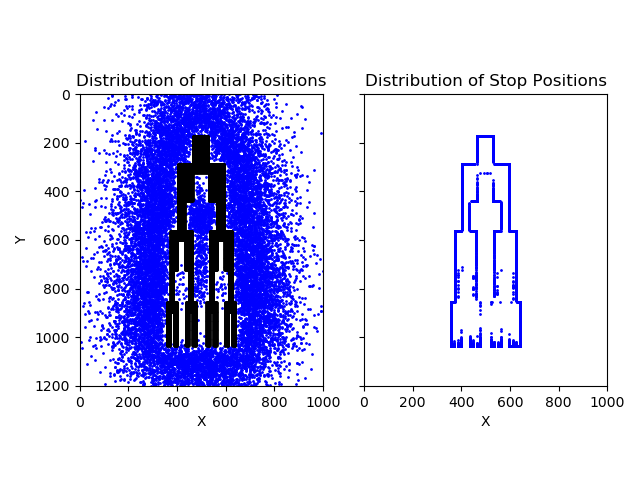
\includegraphics[width=\textwidth]{G_1_L_3_steps_blue_initial_pos_distribution.png}
         \caption{Approximate $15$ percent of particles originally
           started LRWs from the region slightly far away from the
           target object. The number of steps for the blue particles
           is from 4064 to 32586. Not like the
           Fig.~\ref{fig:G_1_L_3_steps_green_initial_pos_distribution},
           fewer blue particles are located initially between the
           narrower branches. Moreover, if particles' initial sites
           are further away from the branching structure's external
           boundary, they will be more dispersive. The particles in
           the right subfigure can depict only some top pieces of the
           internal border.}
         \label{fig:G_1_L_3_steps_blue_initial_pos_distribution}
       \end{figure}
       

       \begin{figure}
         \centering
         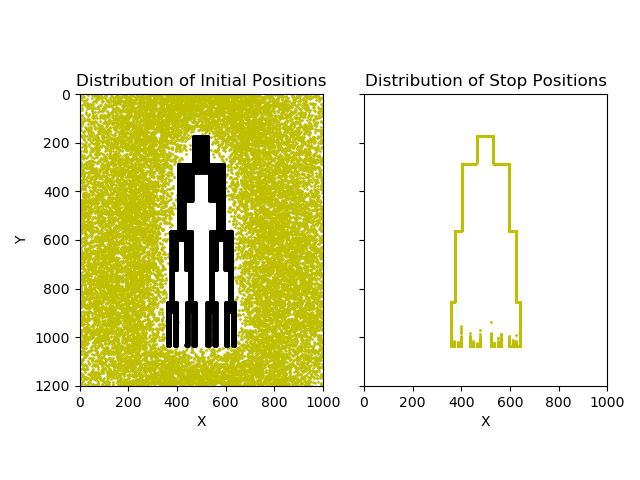
\includegraphics[width=\textwidth]{G_1_L_3_steps_y_initial_pos_distribution.png}
         \caption{The left subplot displays the initial positions of
           $60\%$ of particles in LRWs distributed uniformly in the
           empty space of the image but slightly far away from the
           target object. Moreover, none of them initially started
           LRWs from the in-between region of the branches. Compared
           with the
           Fig.~\ref{fig:G_1_L_3_steps_blue_initial_pos_distribution},
           the right subplot shows the object's entire external
           boundary and some internal boundary of its terminal limbs.}
         \label{fig:G_1_L_3_steps_yellow_initial_pos_distribution}
       \end{figure}


       \begin{figure}
         \centering
         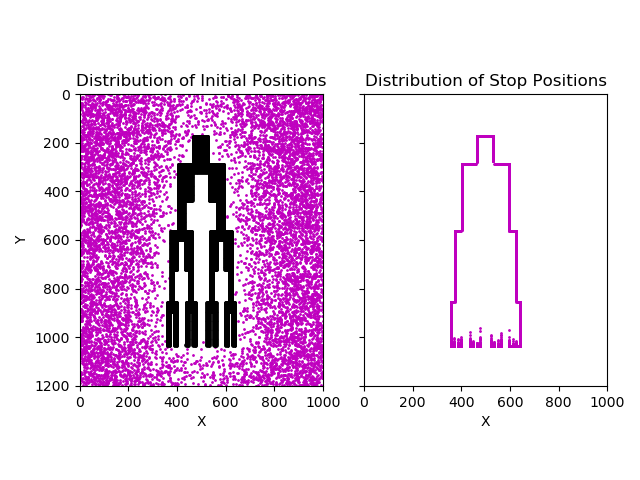
\includegraphics[width=\textwidth]{G_1_L_3_steps_m_initial_pos_distribution.png}
         \caption{Only $10$ percent of particles will survive when
           their number of steps is bigger than $549701$. They are
           distributed initially from a region far away from the
           object and close to the image's edges. Similar to
           Fig.~\ref{fig:G_1_L_3_steps_yellow_initial_pos_distribution},
           pink particles cannot delineate too much internal boundary
           of the branching structure.}
         \label{fig:G_1_L_3_steps_pink_initial_pos_distribution}
       \end{figure}



       In reality, LRWs is latent and cannot be observed
       directly. However, those scatter plots are helpful to reveal
       the first-passage properties of particles in LRWs. For
       instance, particles will be absorbed within a smaller number of
       steps if their starting positions are closer to the target
       because they have less randomness. Moreover, more particles
       will be generated in the broader and longer in-between area of
       branches. Therefore, each segment of the survival curve carries
       massive geometric and spatial information about the unoccupied
       area of the binary image (i.e. the region with black pixels)
       and the boundary of the simply connected domain (i.e. the
       artificial branching structure with white pixels).



       \begin{figure}
        \centering
        \begin{subfigure}[b]{0.45\textwidth}
          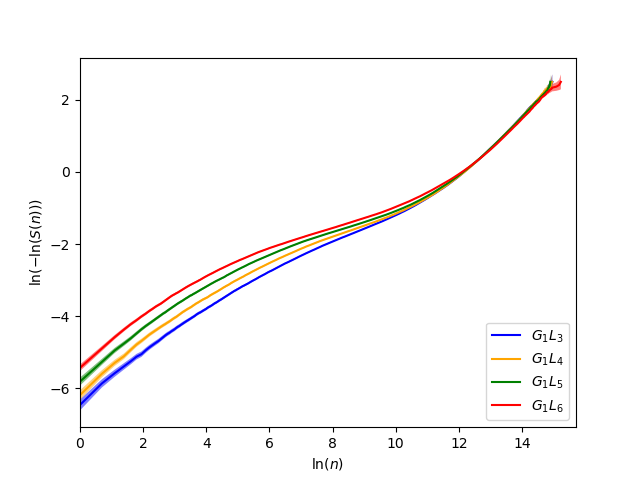
\includegraphics[width=\textwidth]{G_1_steps_check_ph.png}
          \caption{}
          \label{fig:g1_steps_check_ph}
        \end{subfigure}
        \hfill
        \begin{subfigure}[b]{0.45\textwidth}
          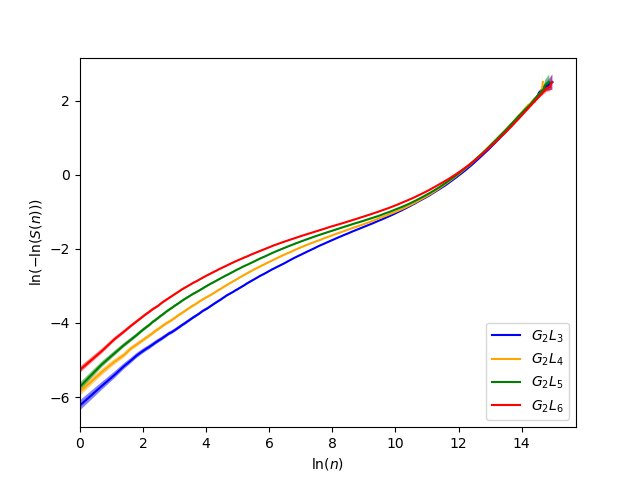
\includegraphics[width=\textwidth]{G_2_steps_check_ph.png}
          \caption{}
          \label{fig:g1_steps_check_ph}
        \end{subfigure}
        \caption{(a) and (b) are commonly used graphical techniques to
          check the proportional hazards (PH) assumption of survival data
          by finding the parallelism. The survival distributions do
          not support the PH assumption since the
          hazard ratio in both $G_1$ and $G_2$ is not always constant.}
        \label{fig:branch_steps_check_ph}
       \end{figure}
       
             
      \begin{table}
        \centering
        \begin{tabular}{llrrrr}
          \toprule
                       &             &         &  p &    &     \\
          \cmidrule{3-6}
                       &             & Log-rank & TW & GB & FH  \\
          \midrule
          $G_1$ $L_3$  & $G_1$ $L_4$  &  0.4393 &  0.0285 &  0.0005 &  0.0005     \\
                       & $G_1$ $L_5$  & 0.0 & 0.0 & 0.0 & 0.0    \\
                       & $G_1$ $L_6$  & 0.0 & 0.0 & 0.0 & 0.0      \\
          $G_1$ $L_4$  & $G_1$ $L_5$  & 0.0007 & 0.0 & 0.0 & 0.0      \\
                       & $G_1$ $L_6$  & 0.0002 & 0.0 & 0.0 & 0.0       \\
          $G_1$ $L_5$   & $G_1$ $L_6$ & 0.7223 &  0.0 & 0.0 & 0.0      \\
          \bottomrule
        \end{tabular}
        \caption{The differences between the pairwise survival
          functions for branching objects in $G_1$ are statistically
          significant based on TW, GB, and FH tests.}
         \label{tab:g1_ingroup_tests_steps}
      \end{table}


      \begin{table}
        \centering
        \begin{tabular}{llrrrr}
          \toprule
                       &             &         &  p &    &     \\
          \cmidrule{3-6}
                       &             & Log-rank & TW & GB & FH  \\
          \midrule
          $G_2$ $L_3$  & $G_2$ $L_4$  &  0.0 &  0.0 &  0.0 &  0.0     \\
                       & $G_2$ $L_5$  & 0.0 & 0.0 & 0.0 & 0.0    \\
                       & $G_2$ $L_6$  & 0.0 & 0.0 & 0.0 & 0.0      \\
          $G_2$ $L_4$  & $G_2$ $L_5$  & 0.0016 & 0.0 & 0.0 & 0.0      \\
                       & $G_2$ $L_6$  & 0.0004 & 0.0 & 0.0 & 0.0       \\
          $G_2$ $L_5$   & $G_2$ $L_6$ & 0.7199 &  0.0 & 0.0 & 0.0      \\
          \bottomrule
        \end{tabular}
        \caption{It is well known that the log-rank test will lose
          power if the proportional hazard assumption is
          violated. Except for the log-rank test, other statistical
          tests indicate that the pairwise survival functions for
          branching objects in $G_2$ are statistically different.}
        \label{tab:g2_ingroup_tests_steps}
      \end{table}
      

      Some weighted log-rank tests can be utilized to detect the early
      or late differences between the pairwise overlapping or crossing
      survival curves. In Table ~\ref{tab:g1_ingroup_tests_steps} and
      Table ~\ref{tab:g2_ingroup_tests_steps}, TW is the abbreviation
      for Tarone-Ware test, GB is for Gehan-Breslow test, and FH is
      for Fleming-Harrington test. However, p values in the tables are
      not too informative, and the log-rank test under conditions of
      non-proportional hazards leads to misleading results. Hence,
      distance measures are alternative methodologies for quantifying
      the discrepancy between survival functions.
      

      It is assumed that $\widehat S_1(t)$ and $\widehat S_2(t)$ are
      the Kaplan-Meier estimators of the survival functions for random
      variable $T_1 > 0$ and $T_2 > 0$, respectively. Let
      $(\tau_j)_{j=1, 2, ..., N}$ are distinct increasing observed
      times when the event of interest take place. In the vector
      space, the distance between $\widehat S_1(t)$ and $\widehat
      S_2(t)$ can be defined as the $L_p$ norm of their difference, $
      1 \leq p \leq \infty$, where

      \begin{equation}\label{eq:lp_norm}
        \begin{split}
          d_p(\widehat S_1(t), \widehat S_2(t))&= \lVert \widehat S_1(t) - \widehat S_2(t) \rVert_{p} \\
          &= \Big(\sum^{N}_{j=1} \lvert \widehat S_1(\tau_j) - \widehat S_2(\tau_j)\rvert^p\Big)^{\frac{1}{p}} \\
          &= \Big(\sum^{N}_{j=1} \lvert P({T_1 > \tau_j}) - P({T_2 > \tau_j}) \rvert^p\Big)^{\frac{1}{p}}
        \end{split}
      \end{equation}
      
      
      \begin{figure}
        \centering
        \begin{subfigure}[b]{0.45\textwidth}
          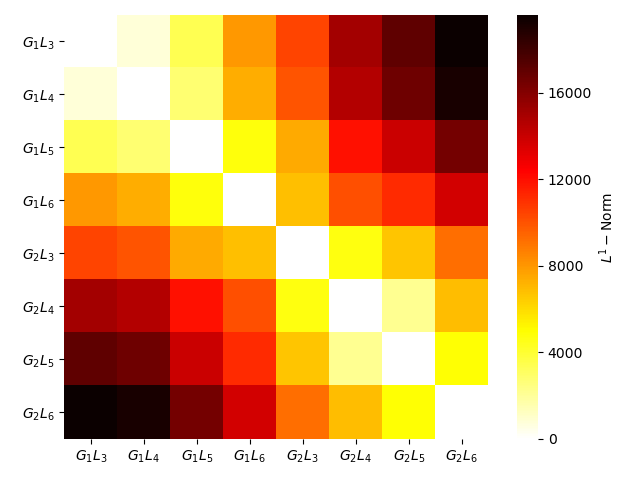
\includegraphics[width=\textwidth]{heatmap_ai_steps_l1.png}
          \caption{}
          \label{fig:heatmap_ai_steps_l1}
        \end{subfigure}
        \begin{subfigure}[b]{0.45\textwidth}
          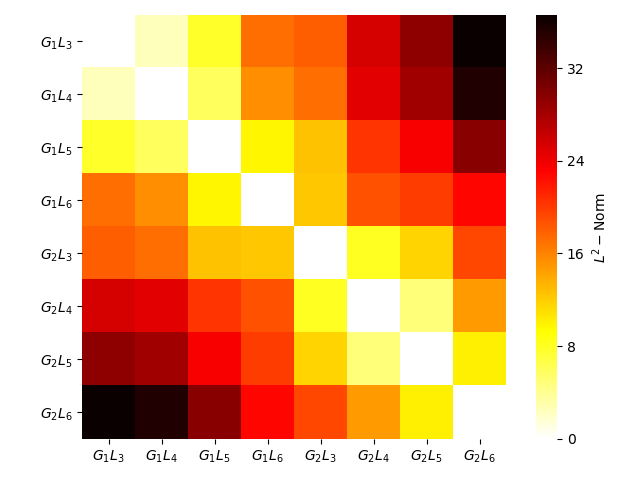
\includegraphics[width=\textwidth]{heatmap_ai_steps_l2.png}
          \caption{}
          \label{fig:heatmap_ai_steps_l2}
        \end{subfigure}
        \caption{The distance matrices of pairwise survival functions for artificial images are visualized by heat maps.}
        \label{fig:heatmap_ai_steps}
      \end{figure}


      Let $p$ be $1$ and $2$ in Eq.~\ref{eq:lp_norm} respectively, the
      distance between a pair of survival functions is measured by
      $d_1$ and $d_2$, and is depicted by colors in the heat maps as
      shown in Fig.~\ref{fig:heatmap_ai_steps_l1} and
      Fig.~\ref{fig:heatmap_ai_steps_l2}. The cells on the main
      diagonal are white because the distance of an object from itself
      is zero. Moreover, the off-diagonal cells are symmetric. The
      darker cells in the heat maps demonstrate more significant
      dissimilarities between survival functions or curves. In other
      words, the colour of cells describes the variation in the shapes
      of branching structures in artificial images.


      The top left and bottom right $4 \times 4$ cells are the
      in-group shape comparison of the branching structures. For each
      column, the cells become darker gradually since the objects in
      each group are more complicated as $j$ increase. The pale yellow
      cells adjacent to the diagonal, including $(G_1L_3, G_1L_4)$,
      $(G_1L_4, G_1L_5)$, $(G_1L_5, G_1L_6)$, $(G_2L_3, G_2L_4)$,
      $(G_2L_4, G_2L_5)$, and $(G_2L_5, G_2L_6)$, imply that the
      morphological changes are not dramatically different. Moreover,
      the top right and bottom left $4 \times 4$ cells are the
      between-group shape comparison. The smaller dissimilarities are
      closer to the diagonal, which gives a form of clustering the
      artificial images.

      
      Metric Multidimensional scaling (MDS) \cite{borg2005modern} is
      employed to display the distance matrix using a map defined in
      an abstract Cartesian space. Given a dimension $p$ and a
      distance matrix $D = (d_{ij})$, MDS is used to find a
      configuration $\bm{x_1}, ..., \bm{x_n} \in \mathbb{R}^p$, which
      satisfies

      \begin{equation}\label{eq:mMDS}
        f(d_{ij}) \approx \widehat{d}_{ij} = \lVert \bm{x_i} - \bm{x_j} \lVert_{2}
      \end{equation}

      as close as possible, and $f$ could be a parametric monotonic function, such as $f(d_{ij}) = \alpha + \beta d_{ij}$.

      Metric MDS aims to minimizes the stress denoted by $\mathcal{L}(\widehat{d}_{ij})$ over all $\widehat{d}_{ij}$, $\alpha$, and $\beta$,

      \begin{equation}\label{eq:stress_mMDS}
        stress = \mathcal{L}(\widehat{d}_{ij}) = \bigg( \sum_{i<j} (\widehat{d}_{ij} - f(d_{ij}))^2 / \sum d^2_{ij} \bigg)^{\frac{1}{2}}
      \end{equation}
      

      In Fig.~\ref{fig:MDS_ai_steps_l1} and
      Fig.~\ref{fig:MDS_ai_steps_l2}, MDS denotes the artificial
      images as points in $2-$ dimensional geometric space so that
      distances between pairs of points match as well as possible the
      original dissimilarities calculated between the pairwise
      survival functions. Moreover, the axes in themselves are
      meaningless. For metric scaling \cite{scikit-learn}, a smaller
      stress $\mathcal{L}(\widehat{d}_{ij})$ indicates a better fit of
      the configuration. Generally, a value of the stress of $20\%$
      suggests a poor fit, $10\%$ fair, $5\%$ good and $2\%$ an
      excellent fit.
       

      \begin{figure}
        \centering
        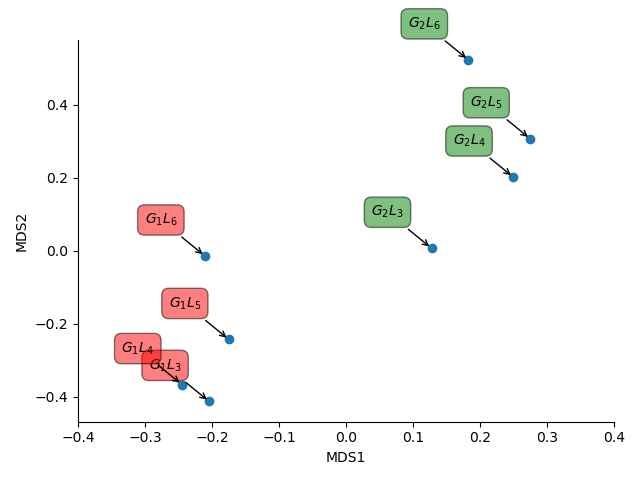
\includegraphics[width=\textwidth]{MDS_ai_steps_l1.png}
        \caption{It is the MDS of the distance matrix calculated based
          on $d_1$, and the stress for the plot is about $0.82\%$. Points
          with green labels in the bottom left-hand corner illustrate
          the $G_1$ images, while others are $G_2$ images. It is easy
          to tell that there are two clusters for the artificial
          images, which coincide with reality and heat map in
          Fig.~\ref{fig:heatmap_ai_steps_l1}.}
        \label{fig:MDS_ai_steps_l1}
      \end{figure}



      \begin{figure}
        \centering
        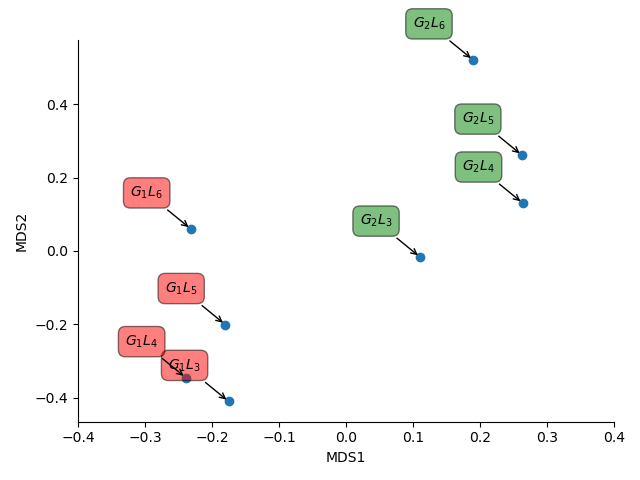
\includegraphics[width=\textwidth]{MDS_ai_steps_l2.png}
        \caption{It is the MDS plot of the distance matrix calculated
          by $d_2$ with the stress $0.4\%$.}
        \label{fig:MDS_ai_steps_l2}
      \end{figure}

      
      



       



       


























      

  
  


\subsection{Output Analysis of $S(d)$}


  \subsubsection{Periodic Boundary Conditions}

      \begin{figure}
         \centering
         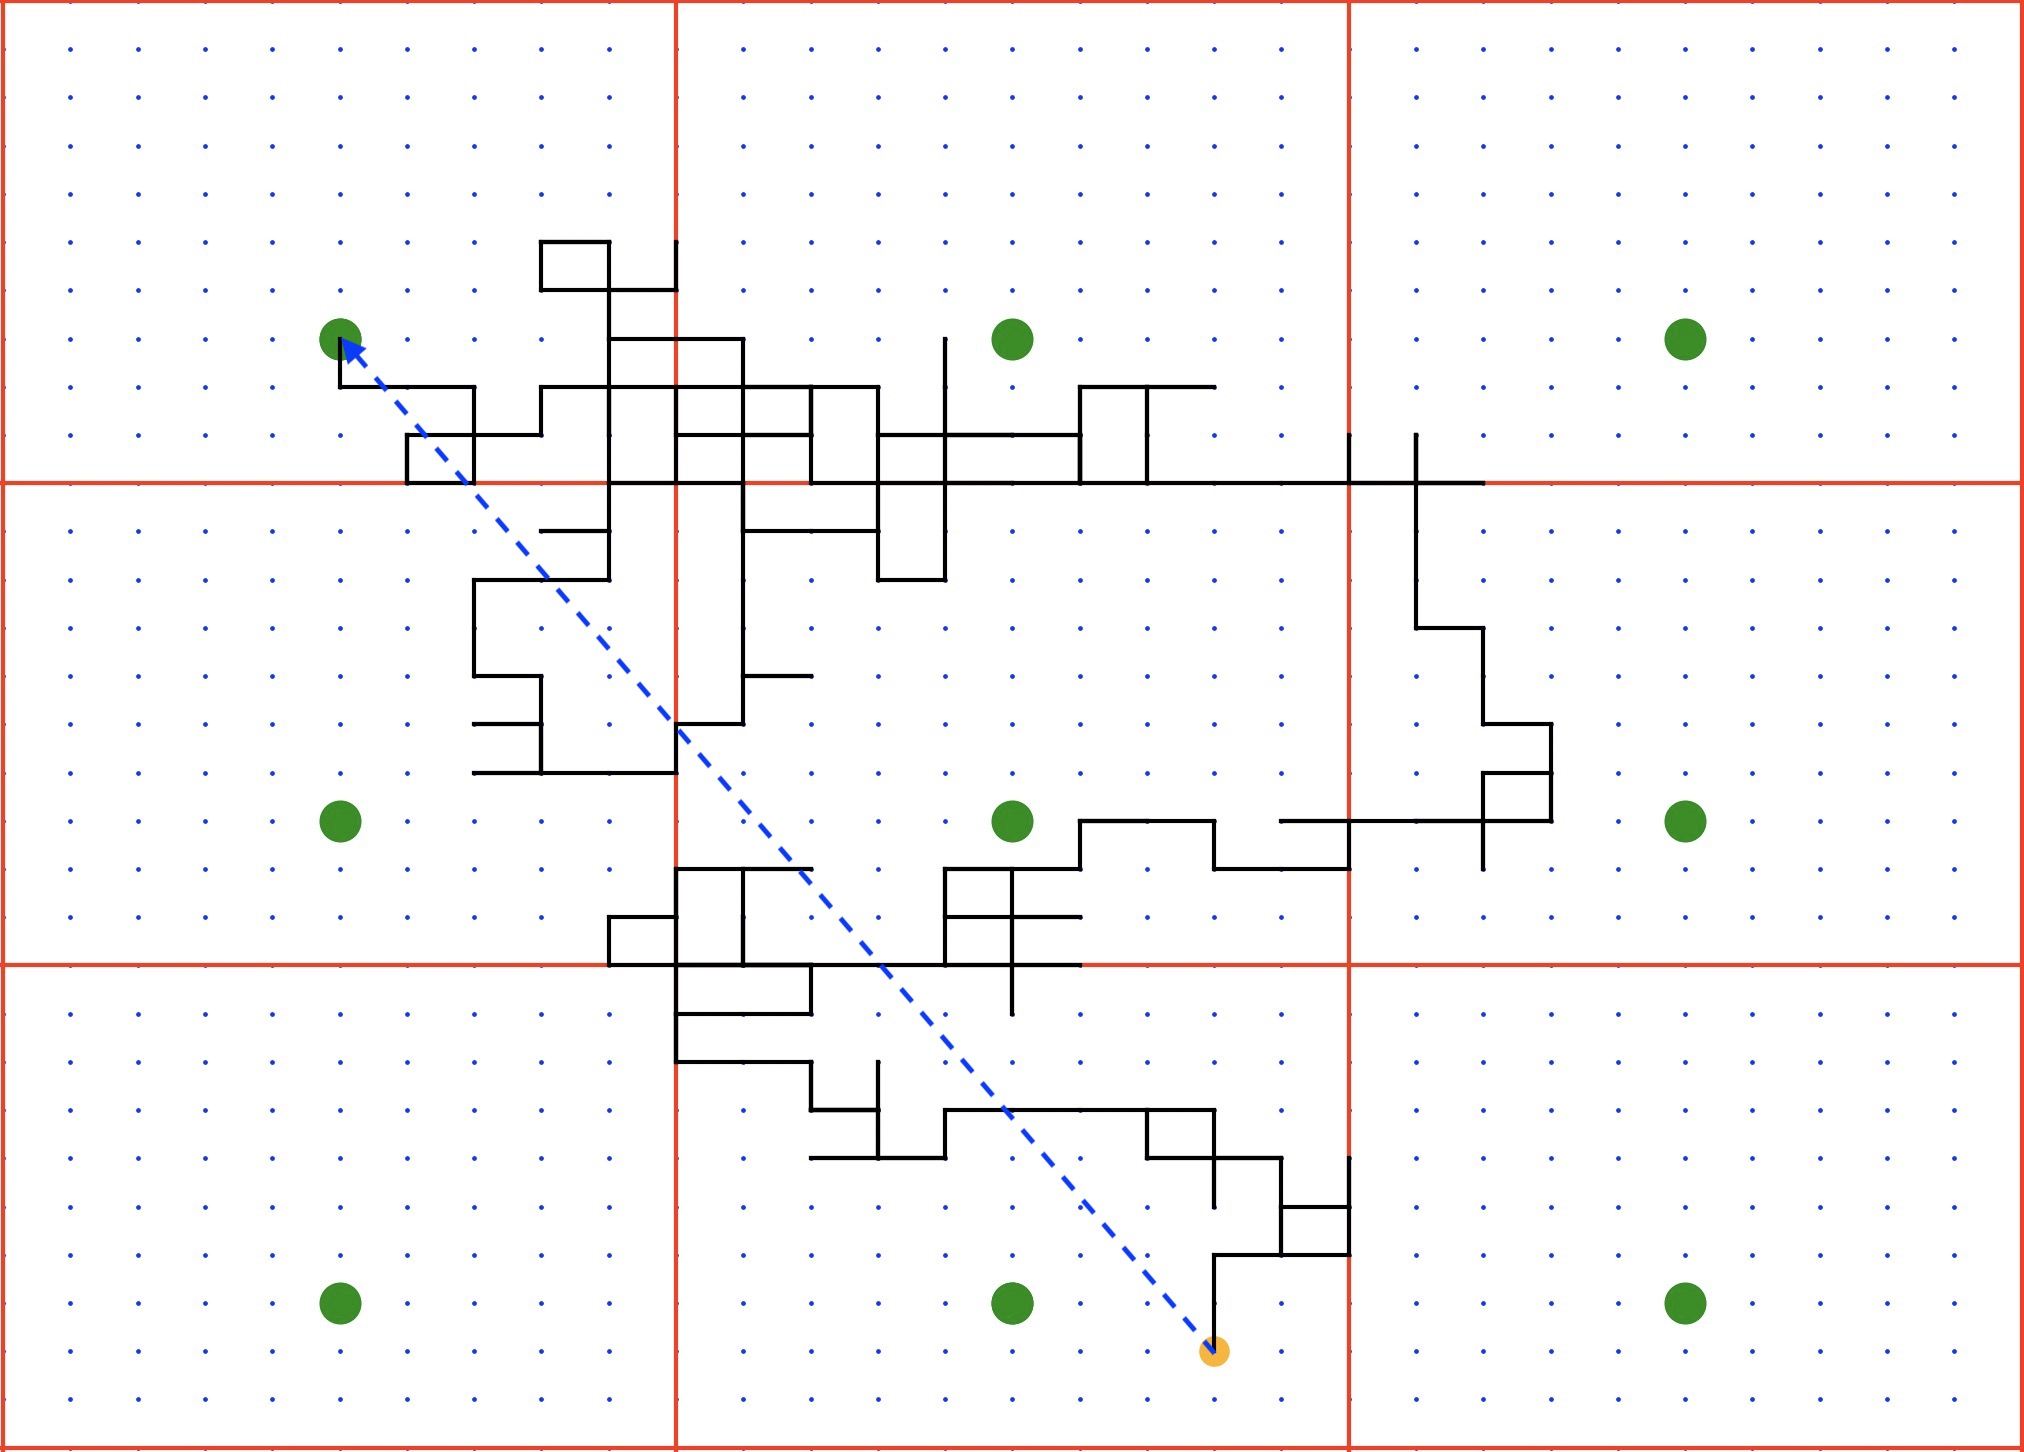
\includegraphics[width=\textwidth]{lrw_perodic_bc.png}
         \caption{This plane is constructed by choosing a primitive
           cell with four red sides and a green point and replicating
           it infinitely to tile the whole $2-$ dimensional
           space. Moreover, there has no overlaps and voids between
           copies of the cell. A particle initially started LRWs from
           the orange site and be absorbed by any of the green points.
           To ensure smoothness and consistency, if the particle
           leaves the cell through one edge, it will appear in the
           adjacent cell with the same velocity. The black line
           segments show the particle's random trajectories, and the
           length of the blue dotted arrow is defined as its
           displacement.}
         \label{fig:pbc_lrws}
      \end{figure}


      In this thesis, periodic boundary conditions (PBCs) are employed
      to minimize the influence of images'
      edges. Fig.~\ref{fig:pbc_lrws} is a simplest example of
      implementing PBCs in the Euclidean plane $E^2$ and tracks the
      trajectory of a particle undergoing LRWs. 




    \subsubsection{Relationship between $n$ and $d$}

     In this section, the displacement of a particle, $d$, is the
     shortest distance from the initial to the stop position in the
     infinite tiling plane. In theory, the mean square displacement
     (MSD) of $N$ Brownian particles at $n-$th step in $2-$dimensional
     space is defined as

     \begin{equation}\label{eq:mds_N}
       MSD = \langle \lvert \bm{r}(n) \lvert^2 \rangle = \frac{1}{N} \sum^{N}_{i=1} (\bm{s}_{i}(n) - \bm{s}_{i}(0))^2 = 4Dn
     \end{equation}
     where the subscript, $i$, refers to each particle for which the
     MSD is calculated. $\bm{s}_{i}(n)$ and $\bm{s}_{i}(0)$ are the
     $i-$th particle positions at $n-$th step and at the initial time,
     respectively. $D$ is diffusion coefficient which is related to
     the variance of the independent displacements of the
     particle. In the simulation, $D$ equals $1$.
     
      
      \begin{figure}
         \centering
         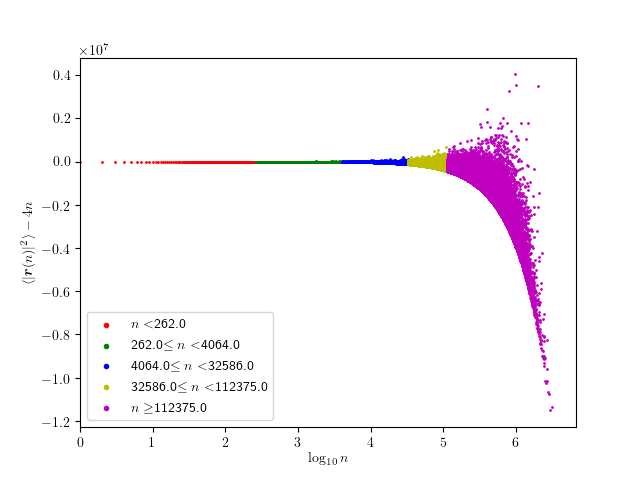
\includegraphics[width=\textwidth]{G_1_L_3_msd_n.png}
         \caption{Particles in $G_1L_3$ are divided into several
           subgroups based on various intervals of steps, and their
           colours are as identical as the segments in
           Fig.~\ref{fig:steps_seg_curve_G_1_L_3}.}
         \label{fig:G_1_L_3_msd_n}
      \end{figure}


     Eq.~\ref{eq:mds_N} indicates a linear relationship between the
     mean square displacement of the particle and the number of
     steps. It is a feature of the normal diffusive
     behavior. Fig.~\ref{fig:G_1_L_3_msd_n} shows how the difference
     between MSD of the particle and $4n$ varying over $\log_{10}n$ in
     LRWs. When $n \leq 4064.0$, the variation is not
     equal to $0$ with larger fluctuation, which implies that blue,
     yellow, and pink particles undergo anomalous diffusion
     process. In other words,

     \begin{equation}\label{eq:anomalous_diffusion}
       \langle \lvert \bm{r}(n) \lvert^2 \rangle \propto n^{\gamma}
     \end{equation}
     where $\gamma \ne 1$. In Fig.~\ref{fig:steps_seg_curve_G_1_L_3},
     negative variation implies $\gamma < 1$ called sub-diffusion
     process, while positive value denotes $\gamma > 1$ named
     super-diffusion.

     
      \begin{figure}
         \centering
         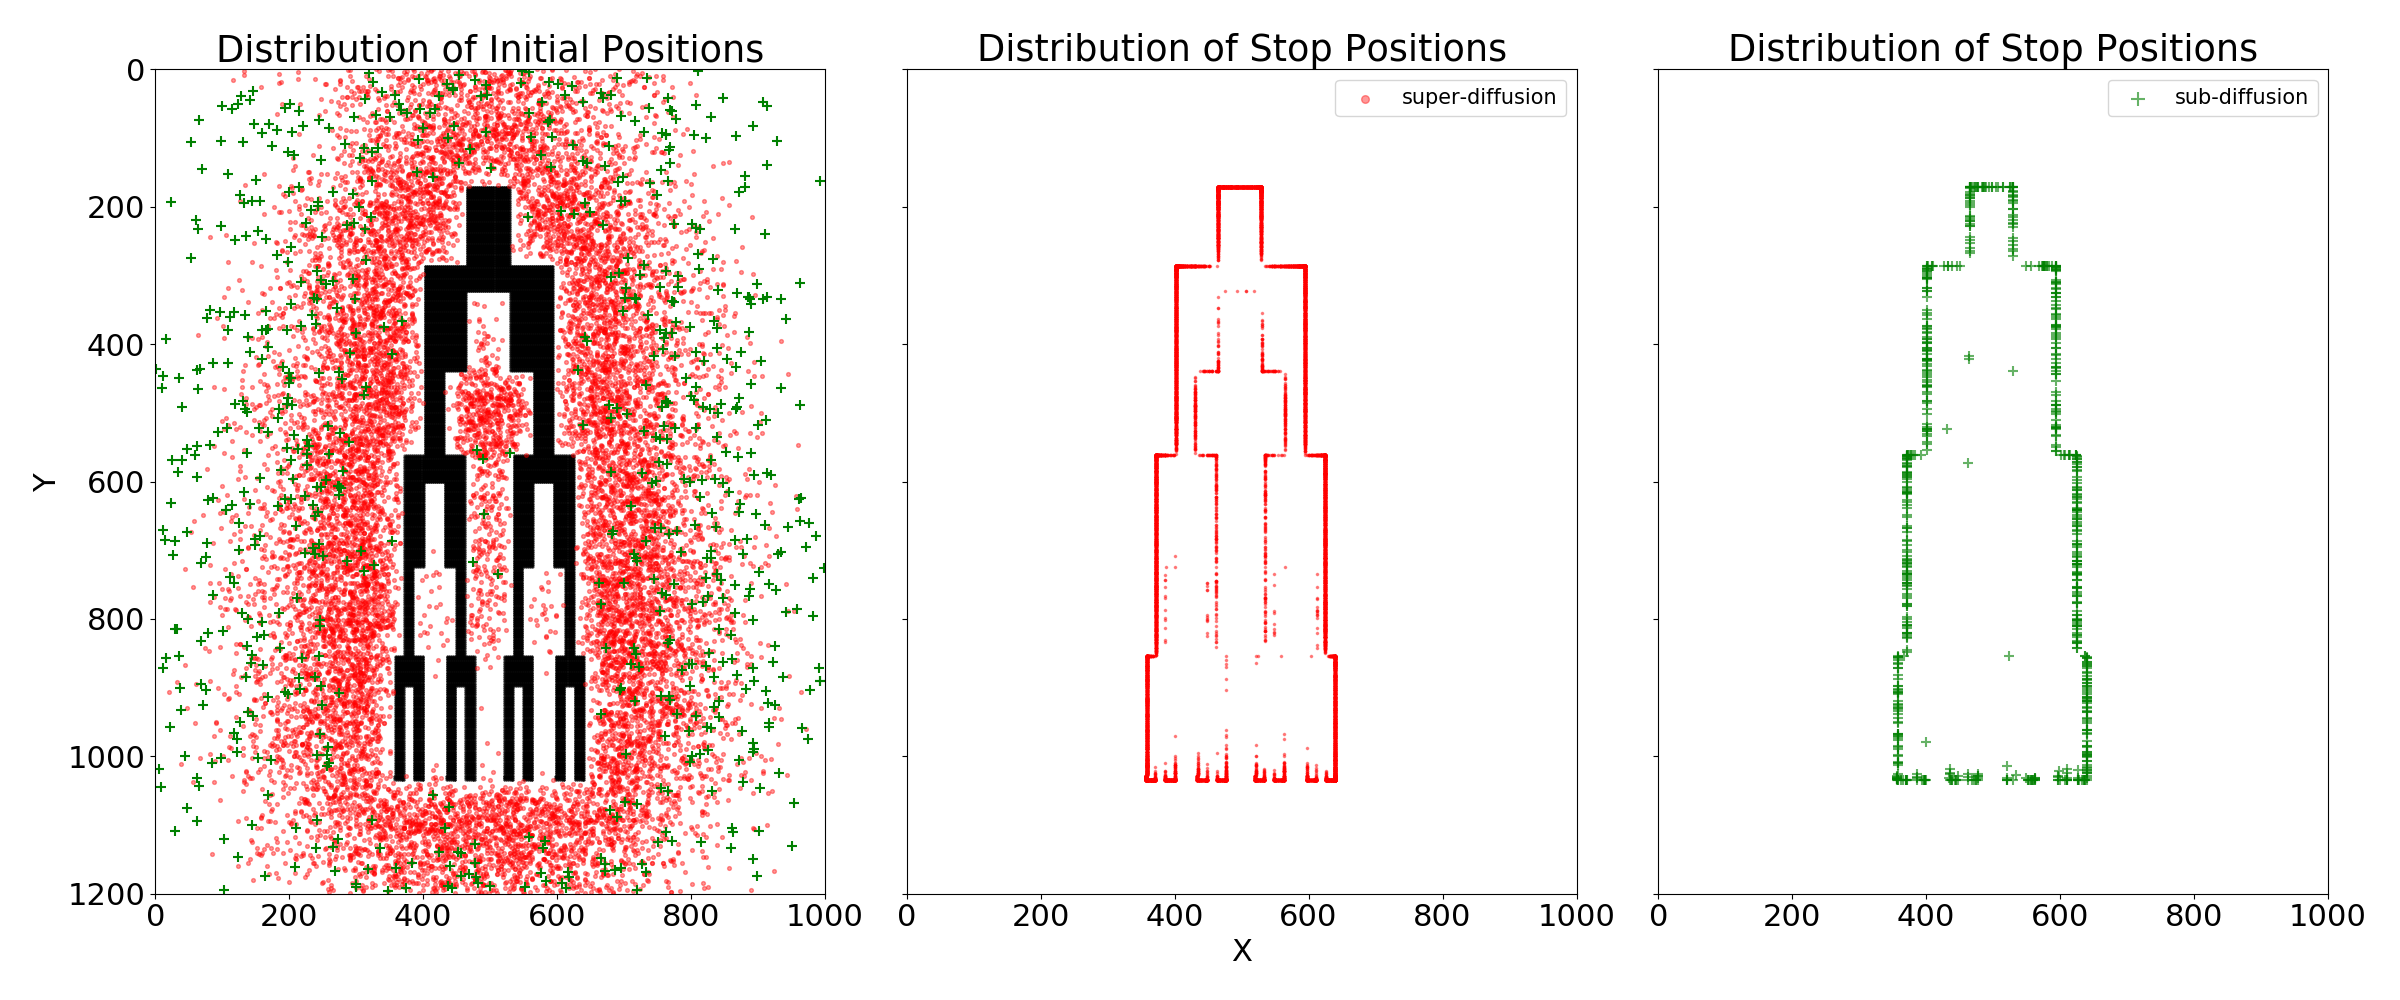
\includegraphics[width=\textwidth]{G_1_L_3_steps_blue_initial_stop_pos_var.png}
         \caption{In the left figure, $696$ dark blue pluses refer to
           super-diffusion particles, which are distributed closer and
           more concentrated to the fringe of the branching
           structure. $15198$ pale blue points represent sub-diffusion
           particles and scatter mainly around the edges of the
           image. In-between the branches, there has only six
           super-diffusion particles and an enormous amount of
           sub-diffusion ones. The middle and right depict the stop
           positions for super and sub-diffusion particles,
           respectively, coloured by a perceptually uniform sequential
           colormap based on their maximum displacement in the tiling
           space.}
         \label{fig:G_1_L_3_var_initial_stop_pos}
      \end{figure}

      To understand the underlying mechanism of the anomalous-type
      diffusion process, initial and stop positions of particles in
      Fig.~\ref{fig:G_1_L_3_steps_blue_initial_pos_distribution},
      whose steps ranged from $4064$ to $32586$, are illustrated in
      Fig.~\ref{fig:G_1_L_3_var_initial_stop_pos}. Suppose particles
      are trapped in the narrow space in-between the branches or
      initially start LRWs near the branching structure. In that case,
      their movements will be restricted because of the nearby
      absorbing boundary condition, causing the sub-diffusion
      phenomenon. As shown in the middle subplot of
      Fig.~\ref{fig:G_1_L_3_var_initial_stop_pos}, the maximum
      displacement of sub-diffusion particles is less than
      $200$. There also have exceptional circumstances that $6$
      particles, in-between the limbs, undergo super-diffusion since
      they can explore a large portion of space within a predefined
      range of steps, as shown in the right subfigure of
      Fig.~\ref{fig:G_1_L_3_var_initial_stop_pos}. Generally,
      particles around the edges of the image will be more likely to
      pass through the periodic boundary, reappear in the adjacent
      cell, and continue LRWs with the same velocity until hitting the
      absorbing boundary, which results in large displacement and the
      super-diffusion process.
      
      

      \subsubsection{Estimated Survival Functions}
      
      \begin{figure}
        \centering
        \begin{subfigure}[b]{0.45\textwidth}
          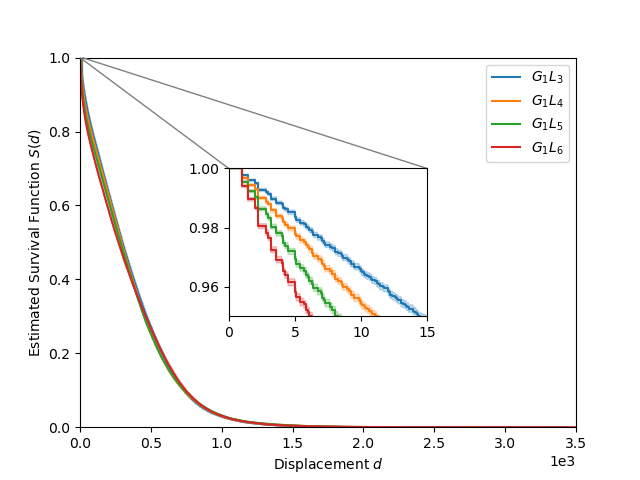
\includegraphics[width=\textwidth]{G_1_unwrap_disp_sf.png}
          \caption{}
          \label{fig:sf_g1_branch_disp}
        \end{subfigure}
        \hfill
        \begin{subfigure}[b]{0.45\textwidth}
          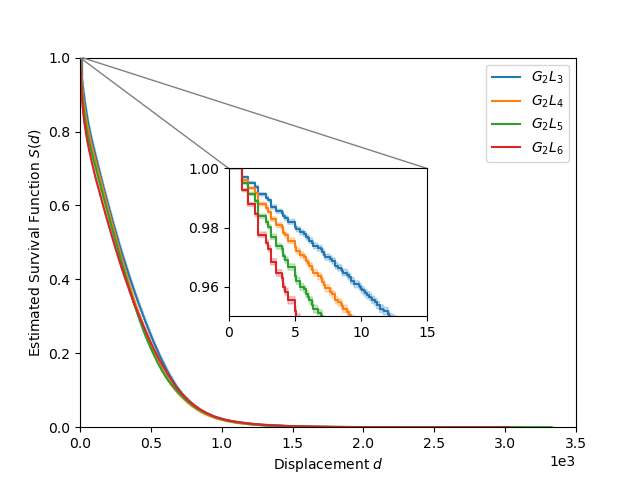
\includegraphics[width=\textwidth]{G_2_unwrap_disp_sf.png}
          \caption{}
          \label{fig:sf_g2_branch_disp}
        \end{subfigure}
        \caption{(a) and (b) are the estimated survival functions
          associated with particles' displacement in LRWs in $G_1$ and
          $G_2$, respectively.}
        \label{fig:sf_branch_disp}
      \end{figure}

      Similar to Fig.~\ref{fig:sf_branch_steps}, it is arduous to
      detect the variation among the survival curves by eyes. However,
      their short-term behaviours can be enlarged in insets in
      Fig.~\ref{fig:sf_branch_disp}, and we can conclude that the
      bigger $L_i$, $i=3, ..., 6$, leads to faster decay of survival
      function. The survival curve is analyzed segment by segment
      based on particles' initial and stop positions, shown in
      Fig.~\ref{fig:G_1_L_3_disp_red_initial_pos_distribution},
      Fig.~\ref{fig:G_1_L_3_disp_green_initial_pos_distribution},
      Fig.~\ref{fig:G_1_L_3_disp_blue_initial_pos_distribution},
      Fig.~\ref{fig:G_1_L_3_disp_yellow_initial_pos_distribution}, and
      Fig.~\ref{fig:G_1_L_3_disp_pink_initial_pos_distribution}, for
      the further understanding.
      


      \begin{figure}
         \centering
         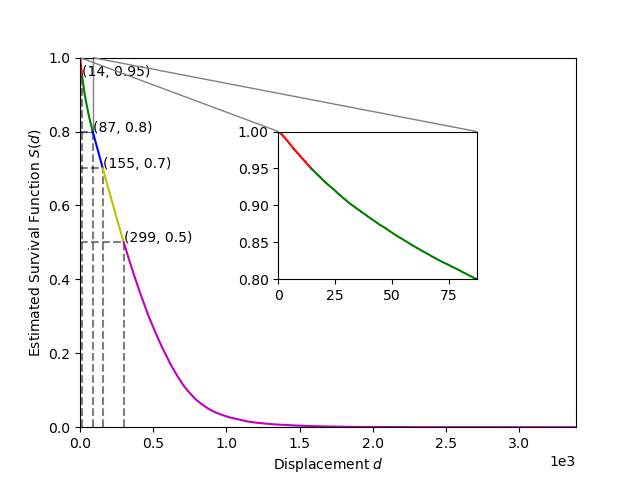
\includegraphics[width=\textwidth]{unwrap_disp_seg_curve_G_1_L_3.png}
         \caption{The estimated survival function is separated into
           five coloured segments based on various intervals of
           displacement. Less than $1\%$ of particles will survive
           when their displacement beyond the height of the image.}
         \label{fig:disp_seg_curve_G_1_L_3}
      \end{figure}

      
       \begin{figure}
         \centering
         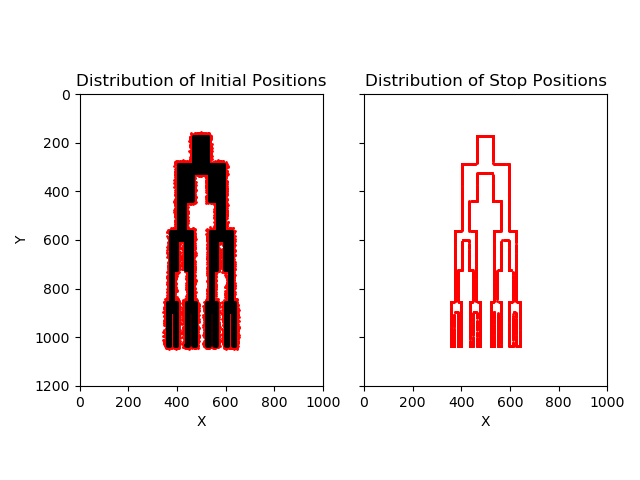
\includegraphics[width=\textwidth]{G_1_L_3_unwrap_disp_red_initial_pos_distribution.png}
         \caption{Five percent of particles are distributed in a tight
           and slender band, with a width of $14$, surrounding the
           branch structure. The area between the bottom and middle
           branches is filled with red particles, which implies the
           vertical spacing between those branches is less than or
           equal to $14$. The right subfigure shows that red particles
           can characterize the entire boundary of the target object.}
         \label{fig:G_1_L_3_disp_red_initial_pos_distribution}
       \end{figure}


       \begin{figure}
         \centering
         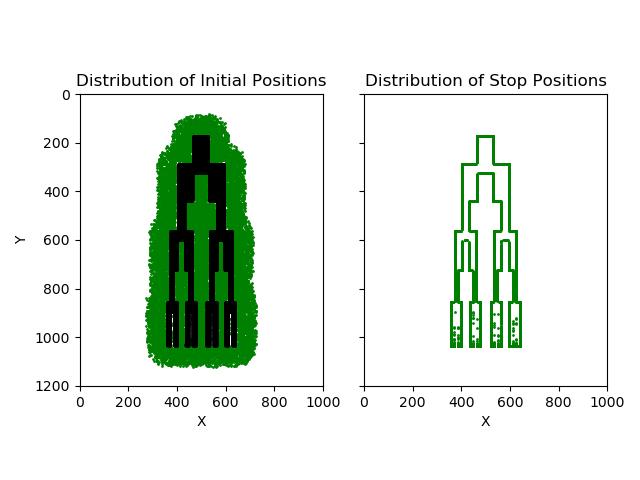
\includegraphics[width=\textwidth]{G_1_L_3_unwrap_disp_green_initial_pos_distribution.png}
         \caption{Compared with
           Fig.~\ref{fig:G_1_L_3_disp_red_initial_pos_distribution},
           fifteen percent of particles can fill the space between the
           branches and occupy the region surrounding the object in
           the shape of a wider band (i.e. with the width
           $73$). Moreover, green particles can not carry the detailed
           information of the boundary of bottom branches.}
         \label{fig:G_1_L_3_disp_green_initial_pos_distribution}
       \end{figure}


        \begin{figure}
         \centering
         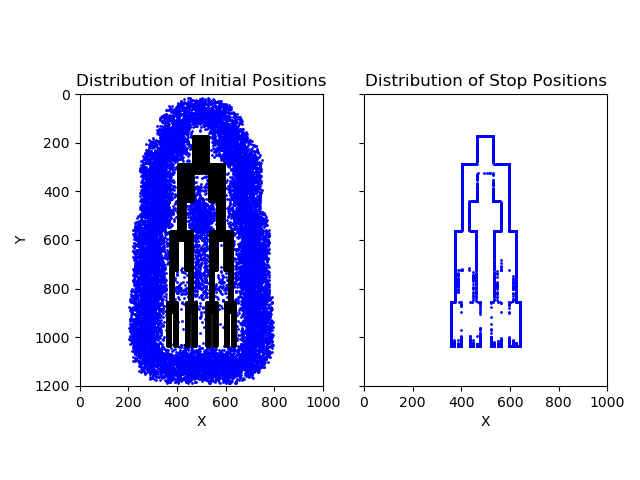
\includegraphics[width=\textwidth]{G_1_L_3_unwrap_disp_blue_initial_pos_distribution.png}
         \caption{Ten percent of particles, whose distances in LRWs
           range between $87$ and $155$, are distributed a little far
           away from the branching structure. Besides, some of them
           are located in the top space between the thick
           branches. Also, the top and bottom of the blue particles
           band are adjacent to the edge of the image. In comparison
           with
           Fig.~\ref{fig:G_1_L_3_disp_green_initial_pos_distribution},
           blue particles show less of the object's internal
           boundary.}
         \label{fig:G_1_L_3_disp_blue_initial_pos_distribution}
        \end{figure}


        \begin{figure}
         \centering
         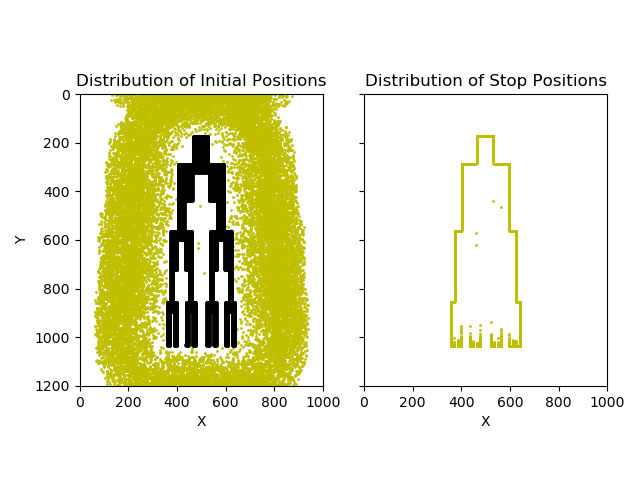
\includegraphics[width=\textwidth]{G_1_L_3_unwrap_disp_y_initial_pos_distribution.png}
         \caption{The irregular yellow domain consists of
           approximately one-fifth of particles whose starting sites
           in the simulation are more remote from the branching
           structure and closer to the borders of the
           image. Nevertheless, there still have a few particles
           between the branches. The yellow area has two notches near
           the top and bottom edge of the image resulting from the
           periodic boundary conditions. Similarly, yellow particles
           only can characterize the external boundary of the target
           object precisely.}
         \label{fig:G_1_L_3_disp_yellow_initial_pos_distribution}
        \end{figure}



        \begin{figure}
         \centering
         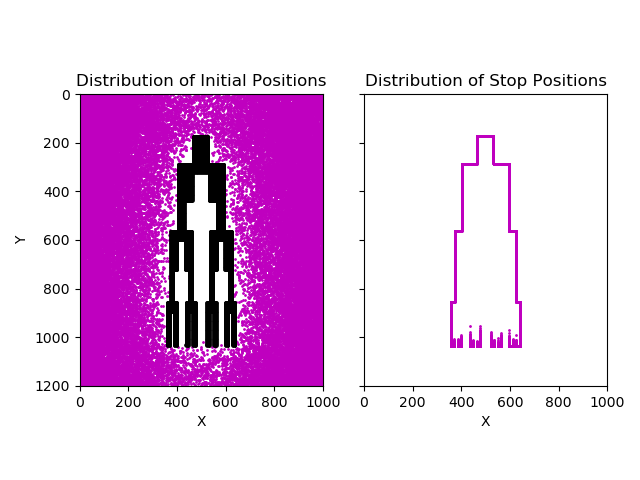
\includegraphics[width=\textwidth]{G_1_L_3_unwrap_disp_m_initial_pos_distribution.png}
         \caption{The rest of the particles fill the unoccupied space
           in the image, but none of them are localized between
           branches. Moreover, pink particles cannot explore the more
           detailed internal boundary of the branching structure
           compared with
           Fig.~\ref{fig:G_1_L_3_disp_yellow_initial_pos_distribution}.}
         \label{fig:G_1_L_3_disp_pink_initial_pos_distribution}
        \end{figure}


        

        \begin{figure}
        \centering
        \begin{subfigure}[b]{0.45\textwidth}
          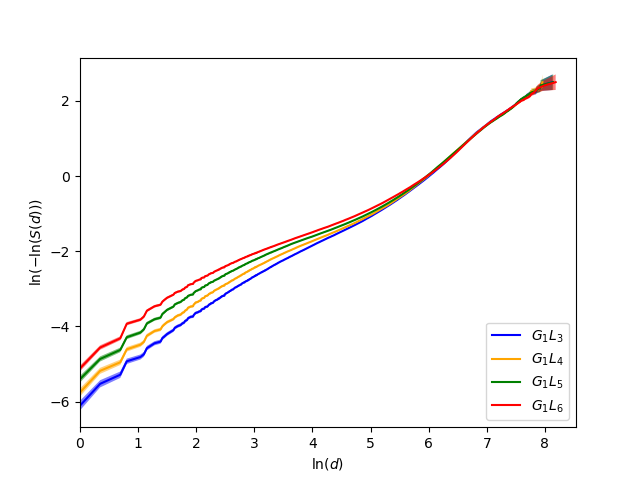
\includegraphics[width=\textwidth]{G_1_unwrap_disp_check_ph.png}
          \caption{}
          \label{fig:g1_disp_check_ph}
        \end{subfigure}
        \hfill
        \begin{subfigure}[b]{0.45\textwidth}
          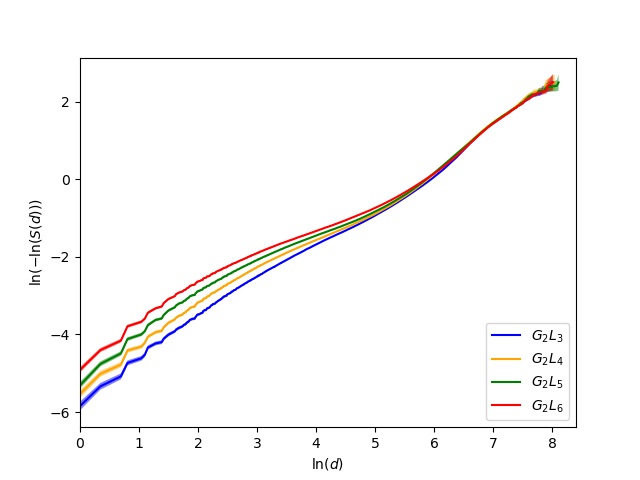
\includegraphics[width=\textwidth]{G_2_unwrap_disp_check_ph.png}
          \caption{}
          \label{fig:g1_disp_check_ph}
        \end{subfigure}
        \caption{}
        \label{fig:branch_disp_check_ph}
      \end{figure}

        
      

      \begin{table}
        \centering
        \begin{tabular}{llrrrr}
          \toprule
                       &             &         &  p &    &     \\
          \cmidrule{3-6}
                       &             & Logrank & TW & GB & FH  \\
          \midrule
          $G_1$ $L_3$  & $G_1$ $L_4$  &  0.0 &  0.0 &  0.0 &  0.0     \\
                       & $G_1$ $L_5$  & 0.0 & 0.0 & 0.0 & 0.0    \\
                       & $G_1$ $L_6$  & 0.0 & 0.0 & 0.0 & 0.0      \\
          $G_1$ $L_4$  & $G_1$ $L_5$  & 0.0072 & 0.0 & 0.0 & 0.0      \\
                       & $G_1$ $L_6$  & 0.0003 & 0.0 & 0.0 & 0.0       \\
          $G_1$ $L_5$   & $G_1$ $L_6$ & 0.2883 &  0.0 & 0.0 & 0.0      \\
          \bottomrule
        \end{tabular}
        \label{tab:g1_ingroup_tests_disp}
        \caption{}
      \end{table}


      \begin{table}
        \centering
        \begin{tabular}{llrrrr}
          \toprule
                       &             &         &  p &    &     \\
          \cmidrule{3-6}
                       &             & Logrank & TW & GB & FH  \\
          \midrule
          $G_2$ $L_3$  & $G_2$ $L_4$  &  0.0 &  0.0 &  0.0 &  0.0     \\
                       & $G_2$ $L_5$  & 0.0 & 0.0 & 0.0 & 0.0    \\
                       & $G_2$ $L_6$  & 0.0 & 0.0 & 0.0 & 0.0      \\
          $G_2$ $L_4$  & $G_2$ $L_5$  & 0.0001 & 0.0 & 0.0 & 0.0      \\
                       & $G_2$ $L_6$  & 0.0015 & 0.0 & 0.0 & 0.0       \\
          $G_2$ $L_5$   & $G_2$ $L_6$ & 0.7019 &  0.0 & 0.0 & 0.0      \\
          \bottomrule
        \end{tabular}
        \label{tab:g2_ingroup_tests_disp}
        \caption{}
      \end{table}



      

      \begin{figure}
        \centering
        \begin{subfigure}[b]{0.45\textwidth}
          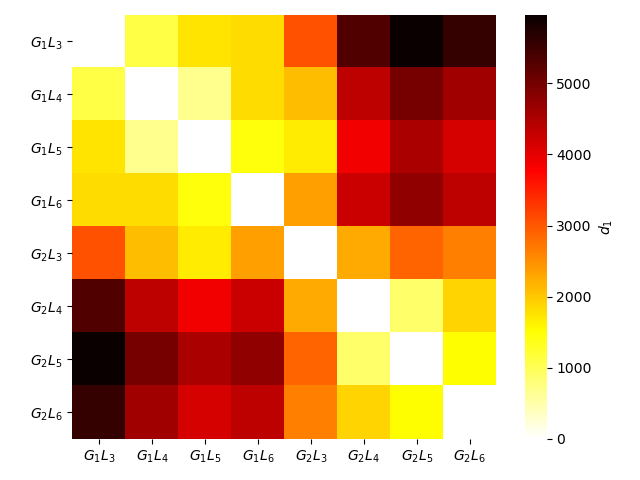
\includegraphics[width=\textwidth]{heatmap_ai_disp_l1.png}
          \caption{}
          \label{fig:heatmap_ai_disp_l1}
        \end{subfigure}
        \begin{subfigure}[b]{0.45\textwidth}
          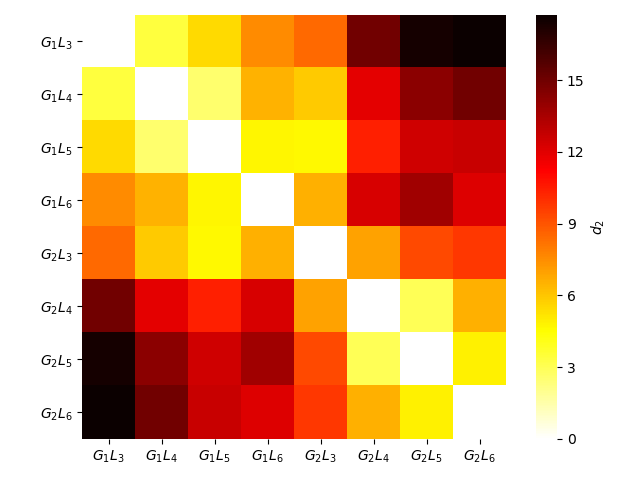
\includegraphics[width=\textwidth]{heatmap_ai_disp_l2.png}
          \caption{}
          \label{fig:heatmap_ai_disp_l2}
        \end{subfigure}
        \caption{}
        \label{fig:heatmap_ai_disp}
      \end{figure}
      

  

\subsection{Output Analysis of $S(R)$}
      
      \begin{figure}
        \centering
        
        \begin{subfigure}[b]{0.45\textwidth}
          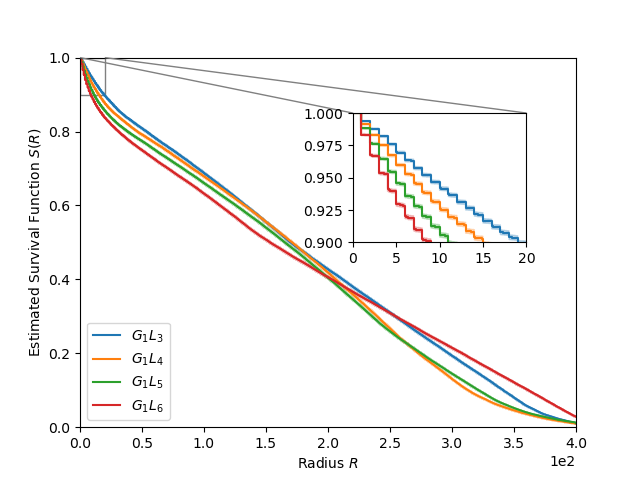
\includegraphics[width=\textwidth]{G_1_initial_radius_sf.png}
          \caption{}
          \label{fig:sf_g1_branch_radius}
        \end{subfigure}
        \hfill
        \begin{subfigure}[b]{0.45\textwidth}
          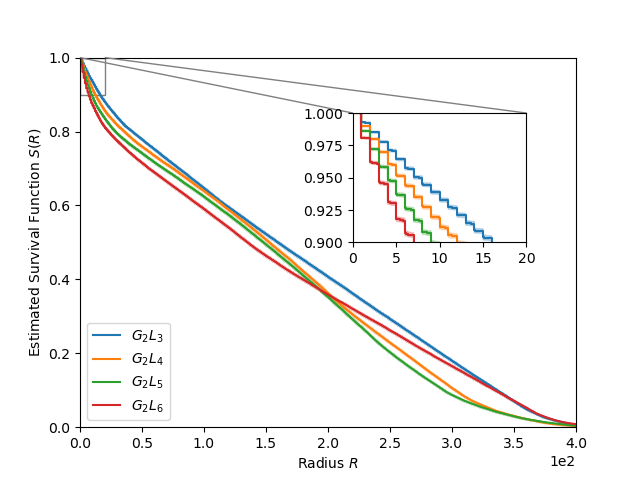
\includegraphics[width=\textwidth]{G_2_initial_radius_sf.png}
          \caption{}
          \label{fig:sf_g2_branch_radius}
        \end{subfigure}

        \caption{}
        \label{fig:sf_branch_radius}

      \end{figure}

      
      \begin{table}
        \centering
        \begin{tabular}{llrrrr}
          \toprule
                       &             &         &  p &    &     \\
          \cmidrule{3-6}
                       &             & Logrank & TW & GB & FH  \\
          \midrule
          $G_1$ $L_3$  & $G_1$ $L_4$  &  0.0 &  0.0 &  0.0 &  0.0     \\
                       & $G_1$ $L_5$  & 0.0 & 0.0 & 0.0 & 0.0    \\
                       & $G_1$ $L_6$  & 0.0 & 0.0 & 0.0 & 0.0      \\
          $G_1$ $L_4$  & $G_1$ $L_5$  & 0.1773 & 0.0 & 0.0 & 0.0      \\
                       & $G_1$ $L_6$  & 0.0 & 0.0 & 0.0 & 0.0       \\
          $G_1$ $L_5$   & $G_1$ $L_6$ & 0.0 &  0.0 & 0.0 & 0.0      \\
          \bottomrule
        \end{tabular}
        \label{tab:g1_ingroup_tests_radius}
        \caption{}
      \end{table}


      \begin{table}
        \centering
        \begin{tabular}{llrrrr}
          \toprule
                       &             &         &  p &    &     \\
          \cmidrule{3-6}
                       &             & Logrank & TW & GB & FH  \\
          \midrule
          $G_2$ $L_3$  & $G_2$ $L_4$  &  0.0 &  0.0 &  0.0 &  0.0     \\
                       & $G_2$ $L_5$  & 0.0 & 0.0 & 0.0 & 0.0    \\
                       & $G_2$ $L_6$  & 0.0 & 0.0 & 0.0 & 0.0      \\
          $G_2$ $L_4$  & $G_2$ $L_5$  & 0.0 & 0.0 & 0.0 & 0.0      \\
                       & $G_2$ $L_6$  & 0.0 & 0.0 & 0.0 & 0.0       \\
          $G_2$ $L_5$   & $G_2$ $L_6$ & 0.0 & 0.0 & 0.0253 & 0.0253      \\
          \bottomrule
        \end{tabular}
        \label{tab:g2_ingroup_tests_radius}
        \caption{}
      \end{table}


      


















  
    \section{Conclusion}

      \begin{itemize}
         \item In a short time, the survival function of rectangle decays faster than the circle, which conforms to the analytical results.
  
         \item The differences of estimated survival functions between circle and rectangle are statistically significant, which coincides with the real shape dissimilarities.

         \item Within a same group, when $t$ is small, the more branching the object is, the faster the survival function decays.

         \item Within a same group, the pairwise survival functions are statistically different.

         \item The corresponding target structures in $G_1$ and $G_3$ are invariant shapes under translation since their survival function are not statistically different. In other words, periodic boundary conditions of the image can eliminate the effect of the locations.

         \item LRWs can describe and classify the geometries, their spatial configurations, and the unoccupied area in the image.
    \end{itemize}


  % _____________ Section 3: Conclusion ________________________
  %\section{Conclusion}\label{section:branch_conclusion}

...



  
  
%%%%%%%%%%%%%%%%%%%%%%%%%% CHAPTER 4 %%%%%%%%%%%%%%%%%%%%%%%%%%%%%%%%%%
\chapter{LRWs in Real Root Images}

 

%%%%%%%%%%%%%%%%%%%%%%%%%% CHAPTER 5 %%%%%%%%%%%%%%%%%%%%%%%%%%%%%%%%%%
\chapter{Conclusion}
  


  
%%%%%%%%%%%%%%%%%%%%%%%%%% CHAPTER 6 %%%%%%%%%%%%%%%%%%%%%%%%%%%%%%%%%%
\chapter{Future Work}

  %___________ Section 1: Conclusion __________________
  %\section{Conclusion}

...




 




% ___________________________ AFTER BODY OF THESIS _________________________

% 12. Referencing Other Works
  % includes quotations, borrowed thoughts or expression


% 13. Appendices
  \uofsappendix % Activate thesis appendix mode

  \begin{appendices}
    
    \chapter{Numerical Methods for Solving Parabolic Partial Differential Equations}
      \section{Introduction}

\begin{itemize}
  \item Parabolic PDEs: to characterize time-dependent phenomena
  \item The intrinsically similar features of the traditional computational techniques are mesh discretization in time and space.
\end{itemize}


\section{Summary of Commonly Used Numerical Techniques}

  \subsection{Finite Difference Method (FDM) \cite{grossmann2007numerical}}

  \subsection{Finite Element Method (FEM) \cite{zlamal1968finite}}

  
  \subsection{Other Tranditional Computational Methods}



\section{Limitation in Practice}


    \chapter{Method Validation in Annulus}
      \section{Analytical Results}


\section{Numerical Approximation}



\section{Comparison of Numerical and Analytical Results}


\section{Conclusion}


    \chapter{Artificial Images}
      

\section{Simple Shapes}


   \begin{figure}[h!]

     \centering
        
        \begin{subfigure}[b]{0.45\textwidth}
          
\includegraphics[width=\textwidth]{circle.png}
          \caption{Circle}
          \label{fig:circle}
        \end{subfigure}
        \hfill
        \begin{subfigure}[b]{0.45\textwidth}
          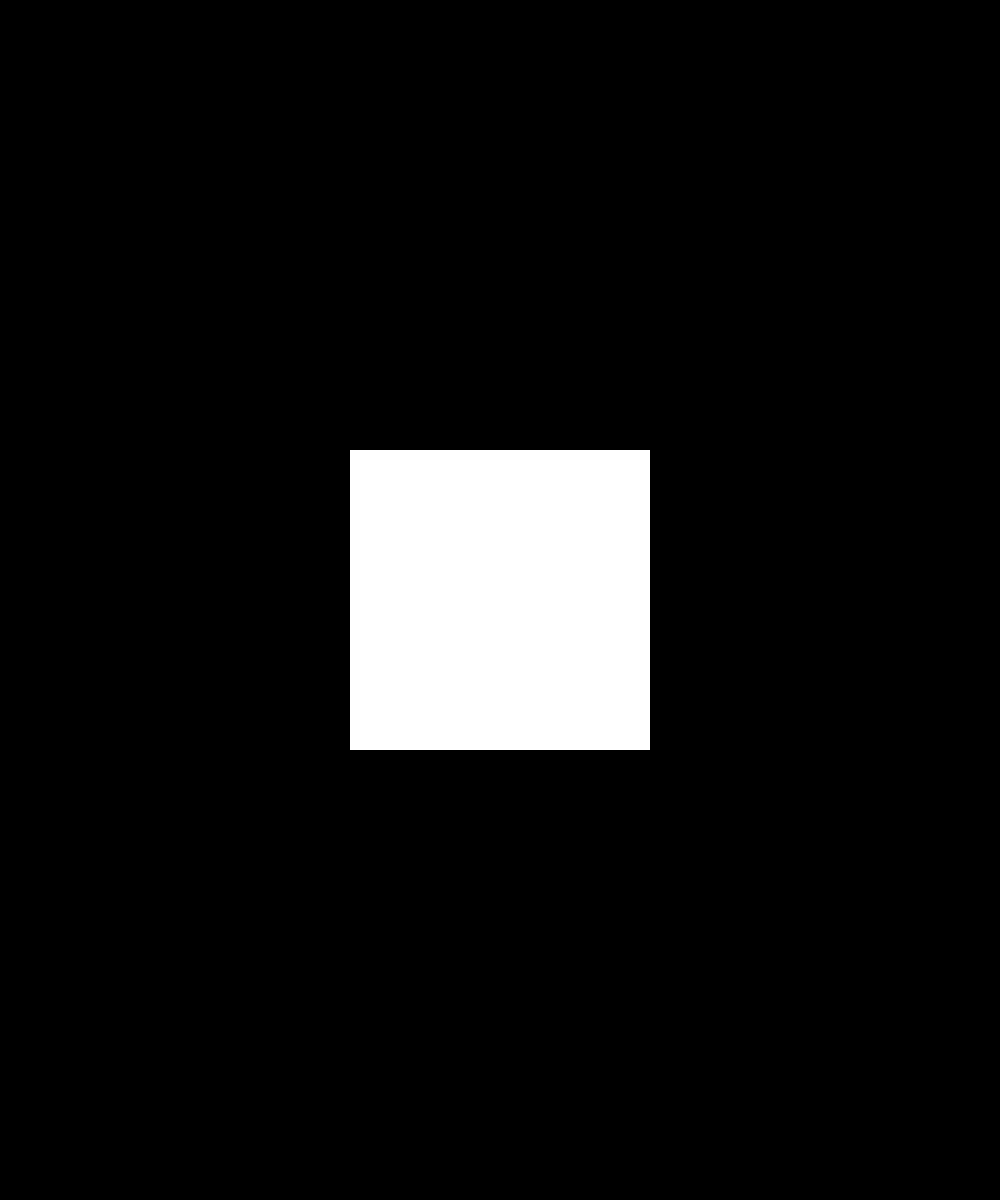
\includegraphics[width=\textwidth]{rectangle.png}
          \caption{Rectangle}
          \label{fig:rectangle}
        \end{subfigure}

        \caption{Each image size is $1200$ by $1000$ pixels with
          $90000$ white pixels.}
        \label{fig:simple_imgs}

   \end{figure}
   



\section{Complicated Branching Structures}

   
    \begin{figure}

     \centering
        
        \begin{subfigure}[b]{0.45\textwidth}
          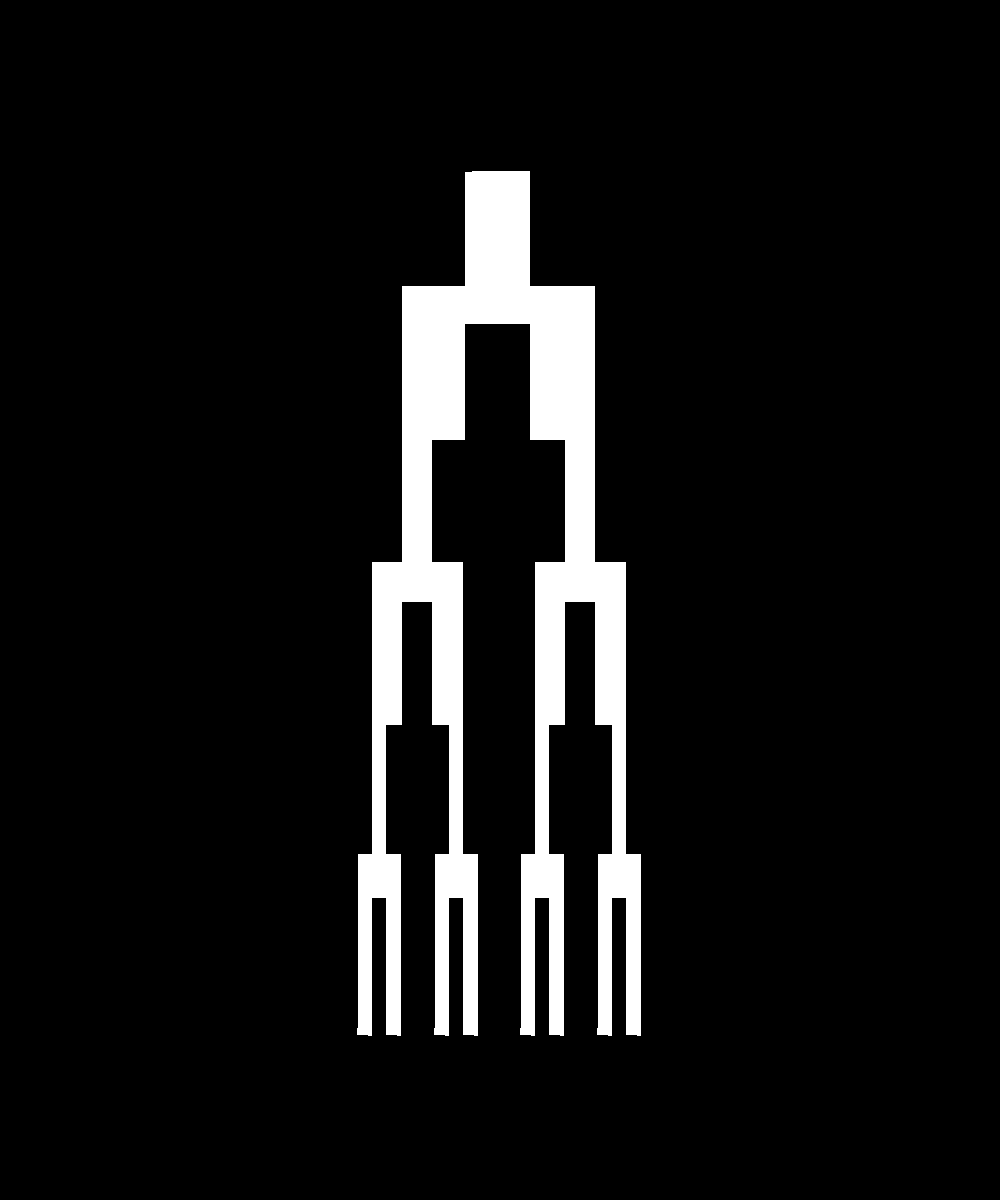
\includegraphics[width=\textwidth]{G_1_L_3.png}
          \caption{$G_1L_3$}
          \label{fig:G1L3}
        \end{subfigure}
        \hfill
        \begin{subfigure}[b]{0.45\textwidth}
          \includegraphics[width=\textwidth]{G_1_L_4.png}
          \caption{$G_1L_4$}
          \label{fig:G1L4}
        \end{subfigure}

        \begin{subfigure}[b]{0.45\textwidth}
          \includegraphics[width=\textwidth]{G_1_L_5.png}
          \caption{$G_1L_5$}
          \label{fig:G1L5}
        \end{subfigure}
        \hfill
        \begin{subfigure}[b]{0.45\textwidth}
          \includegraphics[width=\textwidth]{G_1_L_6.png}
          \caption{$G_1L_6$}
          \label{fig:G1L6}
        \end{subfigure}

        \caption{In the group one, each image size is $1200$ by $1000$ pixels with
          $90000$ white pixels.}
        \label{fig:G1_imgs}

    \end{figure}




    \begin{figure}

     \centering
        
        \begin{subfigure}[b]{0.45\textwidth}
          \includegraphics[width=\textwidth]{G_2_L_3.png}
          \caption{$G_2L_3$}
          \label{fig:G2L3}
        \end{subfigure}
        \hfill
        \begin{subfigure}[b]{0.45\textwidth}
          \includegraphics[width=\textwidth]{G_2_L_4.png}
          \caption{$G_2L_4$}
          \label{fig:G2L4}
        \end{subfigure}

        \begin{subfigure}[b]{0.45\textwidth}
          \includegraphics[width=\textwidth]{G_2_L_5.png}
          \caption{$G_2L_5$}
          \label{fig:G2L5}
        \end{subfigure}
        \hfill
        \begin{subfigure}[b]{0.45\textwidth}
          \includegraphics[width=\textwidth]{G_2_L_6.png}
          \caption{$G_2L_6$}
          \label{fig:G2L6}
        \end{subfigure}

        \caption{In the group two, each image size is $1200$ by $1000$ pixels with
          $90000$ white pixels.}
        \label{fig:G2_imgs}

   \end{figure}


    
  \end{appendices}
  
  

% 14. Referencing and Bibliography
  % should be arranged either alphabetically or numerically
  \uofsbibliography{thesisref}
  %\bibliographystyle{unsrt}


% 15. Electronic Supplements


\end{document}
